% \documentclass{cumcmthesis}

\documentclass[withoutpreface,bwprint]{cumcmthesis} %去掉封面与编号页,电子版提交的时候使用

\usepackage[framemethod=TikZ]{mdframed}
\usepackage{url}   % 网页链接
\usepackage{subcaption} % 子标题
\usepackage{algorithm,algorithmic} % 算法环境
\usepackage[super,square]{natbib} % 引用上标


\begin{document}

%%%%%%%%%%%%%%%%%%%%%%%%%%%%%%%%%%%%%%%%%%%%%%%%%%%%%%%%%%%% 标题 %%%%%%%%%%%%%%%%%%%%%%%%%%%%%%%%%%%%%%%%%%%%%%%%%%%%%%%%%%%%

\title{老外游中国——基于多维数据分析的旅游路线规划模型}
\maketitle

%%%%%%%%%%%%%%%%%%%%%%%%%%%%%%%%%%%%%%%%%%%%%%%%%%%%%%%%%%%% 摘要 %%%%%%%%%%%%%%%%%%%%%%%%%%%%%%%%%%%%%%%%%%%%%%%%%%%%%%%%%%%%
\begin{abstract}
本文针对外国游客在中国境内144小时旅游规划问题,基于包含352个城市景点数据,构建了一系列数学模型进行分析与优化。

对于问题一,通过\textbf{数据挖掘与统计分析方法}对35200个景点评分进行分析,确定了全国景点最高评分为5.0分,共有2563个景点获此评分,其中三沙、五家渠和玉溪等城市拥有最多高评分景点。数据显示,不同城市间景点质量分布存在显著差异。

对于问题二,基于\textbf{加权评价的分析方法},构建了城市吸引力评价体系,综合考虑景点评分、城市中的最佳景点数量和景点游览的时间开销等因素,通过权重分配与综合评分计算,评选出最令外国游客向往的50个城市,为路线规划提供了目的地选择依据。

对于问题三,针对从广州出发的旅游路线规划,构建了\textbf{基于贪心算法的路径优化模型},将问题转化为时间约束下的收益最大化问题。通过迭代计算城市间距离、交通时间和游览价值,在144小时内实现了游览7个城市、62个景点的最优方案,总费用为8353.29元。

对于问题四,通过引入\textbf{多目标优化模型与动态规划算法},将旅游体验与经济成本作为双重目标,重新规划了兼顾城市数量与费用的旅游路线。优化后的方案成功游览9个城市、72个景点,人均景点费用降低至119.84元,较原方案降低了11.05\%,同时提高了景点覆盖率。

对于问题五,针对山景爱好者的特定需求,设计了\textbf{基于遗传算法的主题路线规划模型},通过景点语义分析筛选山景相关景点,从北京出发构建了游览16个城市山景的专题路线,总费用为5574.62元,平均景点评分达4.79分,为特定兴趣游客提供了个性化解决方案。

研究表明,通过\textbf{多维数据分析与多种算法的组合应用},可以有效解决复杂的旅游路线规划问题,为外国游客提供个性化、高效率的中国旅游体验,同时本模型具有较强的扩展性,可应用于不同主题和需求的旅游规划领域。


\keywords{旅游路线规划 \quad 多目标优化 \quad 贪心算法 \quad 动态规划 \quad 遗传算法 \quad 加权评价法}
\end{abstract}


%%%%%%%%%%%%%%%%%%%%%%%%%%%%%%%%%%%%%%%%%%%%%%%%%%%%%%%%%%%% 目录 %%%%%%%%%%%%%%%%%%%%%%%%%%%%%%%%%%%%%%%%%%%%%%%%%%%%%%%%%%%%
\tableofcontents

\newpage % 分页符

%%%%%%%%%%%%%%%%%%%%%%%%%%%%%%%%%%%%%%%%%%%%%%%%%%%%%%%%%%%% 1 问题重述 %%%%%%%%%%%%%%%%%%%%%%%%%%%%%%%%%%%%%%%%%%%%%%%%%%%%%%%%%%%%
\section{问题重述}

%%%%%%%%%%%%%%%%%%%%%%%%%%%%%%%%%%%% 1.1 问题背景 %%%%%%%%%%%%%%%%%%%%%%%%%%%%%%%%%%%%
\subsection{问题背景}
近年来,随着我国过境免签政策的实施和国际交流的日益频繁,越来越多的外国游客选择来中国旅游。
政策允许持联程机票的外国游客无需提前申请签证,即可在限定时间内探索多个城市,
为外国有课在中国的多城联游提供便利\cite{shanghai2013}。



在社交媒体平台上,“City不City”这一网络流行语的传播,
引发了外国游客对中国城市魅力的广泛讨论和浓厚兴趣。
社交媒体提及的“City感”的来源主要为历史文化、自然景观、现代都市或民俗体验(如图\ref{fig:City不City}所示)。

% 结合figure环境添加标题和引用
\begin{figure}[H]
    \centering
    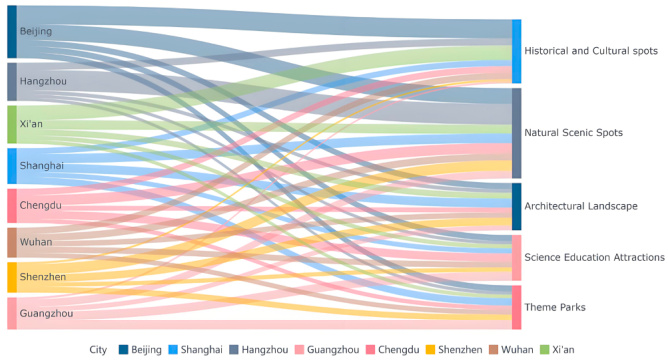
\includegraphics[width=1.0\textwidth]{figures/image/city_city.jpg}
    \caption{社交媒体提及的“City感”城市\cite{sun2024}}
    \label{fig:City不City}
\end{figure}


然而,由于中国地域辽阔、城市众多,外国游客常常面临旅游目的地选择和路线规划的困难。
如何在有限的时间内,游览更多具有代表性的城市,获得最佳的旅游体验,成为一个亟待解决的问题。


本文针对外国游客在中国境内144小时的旅游规划问题,基于包含352个城市、每个城市100个景点的数据集,建立数学模型解决以下问题:
\begin{enumerate}
    \item 分析352个城市中所有35200个景点评分的最高分(BS)及获得该评分的景点数量,并统计拥有最高分景点的城市数量;
    \item 评选出最令外国游客向往的50个城市;
    \item 为从广州入境的外国游客规划144小时内的最佳旅游路线;
    \item 在问题3的基础上,重新规划以降低费用;
    \item 为喜欢山景的外国游客定制旅游路线。
\end{enumerate}

\subsection{问题分析}

\subsubsection{问题分析框架}

本问题涉及多维数据分析和路线规划优化,需要从以下几个方面进行分析:

\begin{enumerate}
    \item \textbf{数据维度分析}
    \begin{itemize}
        \item 景点评分维度:评估景点受欢迎程度的核心指标
        \item 地理空间维度:城市间距离及交通时间成本
        \item 时间维度:游览时间与交通时间的平衡
        \item 成本维度:交通费用与景点门票的综合考量
        \item 特殊偏好维度:针对山景爱好者的定制化需求
    \end{itemize}
    
    \item \textbf{决策模型构建}
    \begin{itemize}
        \item 城市吸引力评估模型:基于景点评分确定城市旅游价值
        \item 路线规划优化模型:在时间约束下最大化旅游体验
        \item 费用优化模型:在保证体验的前提下降低总费用
        \item 特定主题路线规划:针对山景爱好者的专项路线设计
    \end{itemize}
    
    \item \textbf{约束条件分析}
    \begin{itemize}
        \item 时间约束:总游览时间不超过144小时
        \item 起点约束:从广州出发
        \item 景点选择约束:每个城市只选择一个评分最高的景点
        \item 交通方式约束:城市间主要采用高铁交通
    \end{itemize}
    
    \item \textbf{评价指标设计}
    \begin{itemize}
        \item 旅游体验指标:基于城市吸引力和景点评分
        \item 时间效率指标:单位时间内的旅游收益
        \item 成本效益指标:单位成本获得的旅游体验
        \item 特定主题匹配度:山景路线与山景资源的匹配程度
    \end{itemize}
\end{enumerate}
\subsubsection{解决思路}

针对上述问题,我们采取以下解决思路:

\begin{enumerate}
    \item \textbf{数据预处理与分析}
    \begin{itemize}
        \item 清洗和整合352个城市的景点数据
        \item 提取每个景点的评分、位置、游览时间等关键信息
        \item 分析景点评分分布,确定最高分及其分布情况
    \end{itemize}
    
    \item \textbf{城市吸引力评估}
    \begin{itemize}
        \item 基于"城市最佳景点游览原则",提取每个城市评分最高的景点
        \item 构建城市吸引力指数,综合考虑景点评分、评论数等因素
        \item 根据吸引力指数评选出最令外国游客向往的50个城市
    \end{itemize}
    
    \item \textbf{旅游路线规划}
    \begin{itemize}
        \item 构建城市网络图模型,节点为城市,边为城市间连接
        \item 计算城市间距离、交通时间和费用
        \item 设计优化算法,在144小时限制下规划最佳旅游路线
        \item 针对不同优化目标(体验最大化、费用最小化)设计不同策略
    \end{itemize}
    
    \item \textbf{山景旅游路线定制}
    \begin{itemize}
        \item 从景点描述中筛选与山景相关的景点
        \item 重新评估城市吸引力,突出山景资源丰富的城市
        \item 设计专门针对山景爱好者的旅游路线
    \end{itemize}
\end{enumerate}

通过这种系统化的分析框架和解决思路,能够全面解决外国游客在中国境内的旅游规划问题,
提供针对不同需求的最优旅游路线方案。






%%%%%%%%%%%%%%%%%%%%%%%%%%%%%%%%%%%%%%%%%%%%%%%%%%%%%%%%%%%% 2 模型假设 %%%%%%%%%%%%%%%%%%%%%%%%%%%%%%%%%%%%%%%%%%%%%%%%%%%%%%%%%%%%
\section{模型假设}

为了简化问题并使模型具有可行性,我们做出以下假设:
\begin{enumerate}
    \item 假设游客在城市间主要采用高铁交通,平均速度为250km/h\cite{lan2017};
    \item 假设游客每天游览时间为8小时,每个景点平均游览时间根据景点推荐游览时长确定;
    \item 假设景点评分和评论数能够客观反映景点的受欢迎程度\cite{li2021}\cite{kariam2022};
    \item 假设城市间的交通时间和费用与城市之间的直线距离大致成正比\cite{profillidis2013}\cite{colson1914}。
\end{enumerate}


%%%%%%%%%%%%%%%%%%%%%%%%%%%%%%%%%%%%%%%%%%%%%%%%%%%%%%%%%%%% 3 符号说明 %%%%%%%%%%%%%%%%%%%%%%%%%%%%%%%%%%%%%%%%%%%%%%%%%%%%%%%%%%%%
\section{符号说明}

\begin{table}[H]
    \centering
    \begin{tabular}{cl}
        \toprule
        符号 & 含义 \\
        \midrule
        $C$ & 城市集合 \\
        $A_i$ & 城市$i$的景点集合 \\
        $S_{ij}$ & 城市$i$中景点$j$的评分 \\
        $N_{ij}$ & 城市$i$中景点$j$的评论数 \\
        $d_{ij}$ & 城市$i$和城市$j$之间的距离 \\
        $t_{ij}$ & 城市$i$和城市$j$之间的交通时间 \\
        $c_{ij}$ & 城市$i$和城市$j$之间的交通费用 \\
        $V_i$ & 城市$i$的综合旅游价值 \\
        $T$ & 总可用时间(144小时) \\
        $P$ & 最优旅游路线 \\
        \bottomrule
    \end{tabular}

    \caption{符号说明}
    \label{tab:symbols}
\end{table}


%%%%%%%%%%%%%%%%%%%%%%%%%%%%%%%%%%%%%%%%%%%%%%%%%%%%%%%%%%%% 4 模型的建立与求解 %%%%%%%%%%%%%%%%%%%%%%%%%%%%%%%%%%%%%%%%%%%%%%%%%%%%%%%%%%%%
\section{模型的建立与求解}

在本节中,我们将针对外国游客在中国境内旅游的问题,建立一系列数学模型并给出求解过程。
基于"城市最佳景点游览原则",我们设计了多个模型来解决不同方面的问题,包括城市景点评分分析、最佳景点提取、旅游路线规划以及山景旅游路线优化等。

%%%%%%%%%%%%%%%%%%%%%%%%%%%%%%%%%%%% 4.1 城市景点评分分析模型 %%%%%%%%%%%%%%%%%%%%%%%%%%%%%%%%%%%%

\subsection{城市景点评分分析模型}

\subsubsection{模型假设}
\begin{enumerate}
    \item 每个城市的景点评分能够客观反映其吸引力\cite{moraes2013}
    \item 评分为"--"的景点视为无效数据
    \item 城市的整体吸引力与其最高评分景点数量正相关
\end{enumerate}

\subsubsection{模型建立}
我们首先分析各城市景点的评分分布,以确定最受外国游客欢迎的城市。设城市$i$的景点集合为$A_i$,景点$j$的评分为$S_{ij}$,则城市$i$的平均景点评分$\overline{S}_i$为:

\begin{equation}
\overline{S}_i = \frac{\sum_{j=1}^{n_i} S_{ij}}{n_i}
\end{equation}

其中$n_i$为城市$i$的有效景点数量。

为了评估城市对外国游客的吸引力,我们引入"最佳景点指数"(BSI),定义为城市中评分不低于4.5分的景点数量:

\begin{equation}
BSI_i = \sum_{j=1}^{n_i} \mathbb{I}(S_{ij} \geq 4.5)
\end{equation}

其中$\mathbb{I}(\cdot)$为示性函数,当条件满足时取值为1,否则为0。

\subsubsection{求解过程}
我们使用Python读取各城市的景点数据,计算每个城市的平均景点评分和最佳景点指数:

\begin{algorithm}[H]
    \renewcommand{\algorithmicrequire}{\textbf{Input:}}
	\renewcommand{\algorithmicensure}{\textbf{Output:}}
	\caption{Power method}
    \label{power}
    \begin{algorithmic}[1] % 控制是否有序号
    \FOR{每个城市文件}
        \STATE 读取CSV文件中的景点数据
        \STATE 提取有效的评分数据
        \STATE 计算平均评分
        \STATE 统计评分不低于4.5的景点数量
        \STATE 更新城市最佳景点计数
    \ENDFOR
\end{algorithmic}
\end{algorithm}

\subsubsection{结果分析}
通过计算,可以得到各城市的平均景点评分和最佳景点指数。
结果显示,全国有 2563 个景点获评最高评分(BS),三沙、五家渠、玉溪、益阳、天门、大兴安岭等城市拥有较多的高评分景点,这些城市对游客具有较强的吸引力。
具体来说,排名前10的城市及其最佳景点指数如表\ref{tab:best_scores} 所示:

\begin{table}[H]
\centering
\caption{城市最佳景点指数排名}
\label{tab:best_scores}
\begin{tabular}{ccc}
\hline
排名 & 城市 & 最佳景点指数 \\
\hline
1 & 三沙 & 36 \\
2 & 五家渠 & 28 \\
3 & 玉溪 & 21 \\
4 & 益阳 & 20 \\
5 & 天门 & 19 \\
6 & 大兴安岭 & 18 \\
7 & 潍坊 & 18 \\
8 & 烟台 & 18 \\
9 & 阿拉尔 & 18 \\
10 & 邢台 & 17 \\
\hline
\end{tabular}
\end{table}




%%%%%%%%%%%%%%%%%%%%%%%%%%%%%%%%%%%% 4.2 最佳景点提取模型 %%%%%%%%%%%%%%%%%%%%%%%%%%%%%%%%%%%%

\subsection{最佳景点提取模型}

\subsubsection{模型假设}
\begin{enumerate}
    \item 每个城市只选择一个评分最高的景点进行游览
    \item 当多个景点评分相同且最高时,优先选择游览时间较短的景点
    \item 景点游览时间可以通过"建议游览时间"字段估算
\end{enumerate}

\subsubsection{模型建立}
对于每个城市$i$,我们需要从其景点集合$A_i$中选择最佳景点$a_i^*$,选择标准为:

\begin{equation}
a_i^* = \arg\max_{j \in A_i} S_{ij}
\end{equation}

当存在多个评分相同的最高分景点时,我们选择游览时间较短的景点:

\begin{equation}
a_i^* = \arg\min_{j \in A_i^*} T_{ij}
\end{equation}

其中$A_i^*$为城市$i$中评分最高的景点子集,$T_{ij}$为景点$j$的游览时间。

\subsubsection{求解过程}
我们通过以下步骤提取每个城市的最佳景点:

\begin{algorithm}[!ht]
    \renewcommand{\algorithmicrequire}{\textbf{Input:}}
	\renewcommand{\algorithmicensure}{\textbf{Output:}}
	\caption{Power method}
    \label{power}
    \begin{algorithmic}[1] % 控制是否有序号
\FOR{每个城市文件}
    \STATE 读取CSV文件中的景点数据
    \STATE 按评分降序排序
    \STATE 选择评分最高的景点
    \IF{存在多个评分相同的最高分景点}
        \STATE 计算每个景点的游览时间
        \STATE 选择游览时间最短的景点
    \ENDIF
    \STATE 保存最佳景点信息
\ENDFOR
\end{algorithmic}
\end{algorithm}

为了准确估算景点的游览时间,我们开发了一个文本解析函数,将"建议游览时间"字段转换为小时数:

\begin{equation}
T_{ij} = \begin{cases}
h, & \text{如果建议时间为$h$小时} \\
\frac{h_1 + h_2}{2}, & \text{如果建议时间为$h_1-h_2$小时} \\
24h, & \text{如果建议时间为$h$天} \\
24, & \text{如果无建议时间}
\end{cases}
\end{equation}

\subsubsection{结果分析}
通过该模型,我们成功提取了“最令外国游客向往的 50 个城市”以及这 50 个城市中每个城市的最佳景点。

“最令外国游客向往的 50 个城市”城市分别为:三沙、五家渠、玉溪、益阳、天门、烟台、可克达拉、大兴安岭、潍坊、阿拉尔、
雅安、邢台、保亭、周口、自贡、内江、万宁、庆阳、沈阳、保定、
东营、阳泉、宁德、德州、抚州、武威、泸州、廊坊、商丘、昭通、
淮北、贵港、郴州、伊犁、凉山、保山、大庆、无锡、芜湖、齐齐哈尔、
江门、临汾、六安、商洛、塔城、娄底、定西、宿州、德阳、本溪。

结果显示,不同城市的最佳景点类型多样,包括历史文化景点与自然风光等。
历史文化景点如:天门的陆羽纪念馆、潍坊的郭味蕖故居陈列馆、雅安的清代立交桥等;
自然风光如:三沙的北礁、烟台的宝塔礁、保亭的七仙岭温泉等。

这些最佳景点将作为外国游客在各城市游览的首选目的地。
我们将这些景点信息整合到一个数据集中,为后续的旅游路线规划提供基础数据。

%%%%%%%%%%%%%%%%%%%%%%%%%%%%%%%%%%%% 4.3 旅游路线规划模型 %%%%%%%%%%%%%%%%%%%%%%%%%%%%%%%%%%%%

\subsection{旅游路线规划模型}

\subsubsection{模型假设}
\begin{enumerate}
    \item 游客在144小时内可以游览多个城市
    \item 城市间交通采用高铁,平均速度为250km/h
    \item 城市的吸引力与其在外国游客向往城市排名中的位置相关
    \item 游览一个城市的时间与其吸引力正相关
\end{enumerate}

\subsubsection{模型建立}
我们将旅游路线规划问题建模为一个有约束的最优化问题。设城市集合为$C = \{c_1, c_2, \ldots, c_n\}$,起始城市为$c_s$,我们需要找到一条路径$P = (c_s, c_{i_1}, c_{i_2}, \ldots, c_{i_k})$,使得:

\begin{equation}
\max \sum_{c_i \in P} A(c_i)
\end{equation}

其中$A(c_i)$表示城市$c_i$的吸引力得分,定义为:

\begin{equation}
A(c_i) = \begin{cases}
51 - r_i, & \text{如果$c_i$在前50名城市中} \\
0, & \text{其他情况}
\end{cases}
\end{equation}

其中$r_i$为城市$c_i$在外国游客向往城市排名中的位置。

约束条件为总时间不超过144小时:

\begin{equation}
\sum_{c_i \in P} V(c_i) + \sum_{j=1}^{k} T(c_{i_{j-1}}, c_{i_j}) \leq 144
\end{equation}

其中$V(c_i)$为游览城市$c_i$所需的时间,$T(c_i, c_j)$为从城市$c_i$到城市$c_j$的交通时间,计算公式为:

\begin{equation}
T(c_i, c_j) = \frac{D(c_i, c_j)}{250}
\end{equation}

其中$D(c_i, c_j)$为两城市间的距离(公里),使用Haversine公式计算:

\begin{equation}
D(c_i, c_j) = 2R \cdot \arcsin\left(\sqrt{\sin^2\left(\frac{\phi_j - \phi_i}{2}\right) + \cos(\phi_i)\cos(\phi_j)\sin^2\left(\frac{\lambda_j - \lambda_i}{2}\right)}\right)
\end{equation}

其中$R$为地球的平均半径(6371公里),$\phi_i$和$\lambda_i$分别为城市$c_i$的纬度和经度(弧度)。

\subsubsection{求解过程}
我们采用贪心算法求解该最优化问题\cite{xiang2022}:

\begin{algorithm}[H]
    \renewcommand{\algorithmicrequire}{\textbf{Input:}}
	\renewcommand{\algorithmicensure}{\textbf{Output:}}
	\caption{Power method}
    \label{power}
    \begin{algorithmic}[1] % 控制是否有序号
\STATE 初始化路径$P = (c_s)$,剩余时间$T_r = 144$
\WHILE{$T_r > 0$}
    \STATE 找到未访问城市$c_j$,使得$\frac{A(c_j)}{V(c_j) + T(c_{last}, c_j)}$最大
    \IF{$V(c_j) + T(c_{last}, c_j) \leq T_r$}
        \STATE 将$c_j$添加到路径$P$中
        \STATE $T_r = T_r - V(c_j) - T(c_{last}, c_j)$
    \ELSE
        \STATE 跳出循环
    \ENDIF
\ENDWHILE
\end{algorithmic}
\end{algorithm}

\subsubsection{结果分析}

如表\ref{tab:最佳旅游路线规划}、图\ref{fig:最佳旅游路线示意图}所示,通过上述模型可以得到一条优化的旅游路线,
使得外国游客能够在144小时内游览尽可能多的高吸引力城市。

\begin{table}[H]
  \centering
  \caption{最佳旅游路线规划}
  \label{tab:最佳旅游路线规划}
  \begin{tabular}{|c|c|c|c|c|c|}
    \hline
    \textbf{城市} & \textbf{交通方式} & \textbf{交通时间(小时)} & \textbf{交通费用(元)} & \textbf{景点数量} & \textbf{门票费用(元)} \\
    \hline
    广州(起点) & - & - & - & 2 & 67 \\
    \hline
    郴州 & 高铁(从广州) & 6.0 & 694 & 8 & 200 \\
    \hline
    自贡 & 高铁(从郴州) & 14.0 & 1590 & 12 & 20 \\
    \hline
    廊坊 & 高铁(从自贡) & 9.3 & 1069 & 10 & 300 \\
    \hline
    周口 & 高铁(从廊坊) & 23.3 & 2636 & 12 & 400 \\
    \hline
    德州 & 高铁(从周口) & 7.1 & 820 & 10 & 300 \\
    \hline
    塔城 & 高铁(从德州) & 2.0 & 242 & 8 & 15 \\
    \hline
    \multicolumn{2}{|c|}{\textbf{总计}} & \textbf{61.7} & \textbf{7051} & \textbf{62} & \textbf{1302.29} \\
    \hline
    \multicolumn{5}{|c|}{\textbf{总游玩时间(小时)}} & \textbf{143.61} \\
    \hline
    \multicolumn{5}{|c|}{\textbf{总费用(元)}} & \textbf{8353.29} \\
    \hline
  \end{tabular}
\end{table}

\begin{figure}[H]
    \centering
    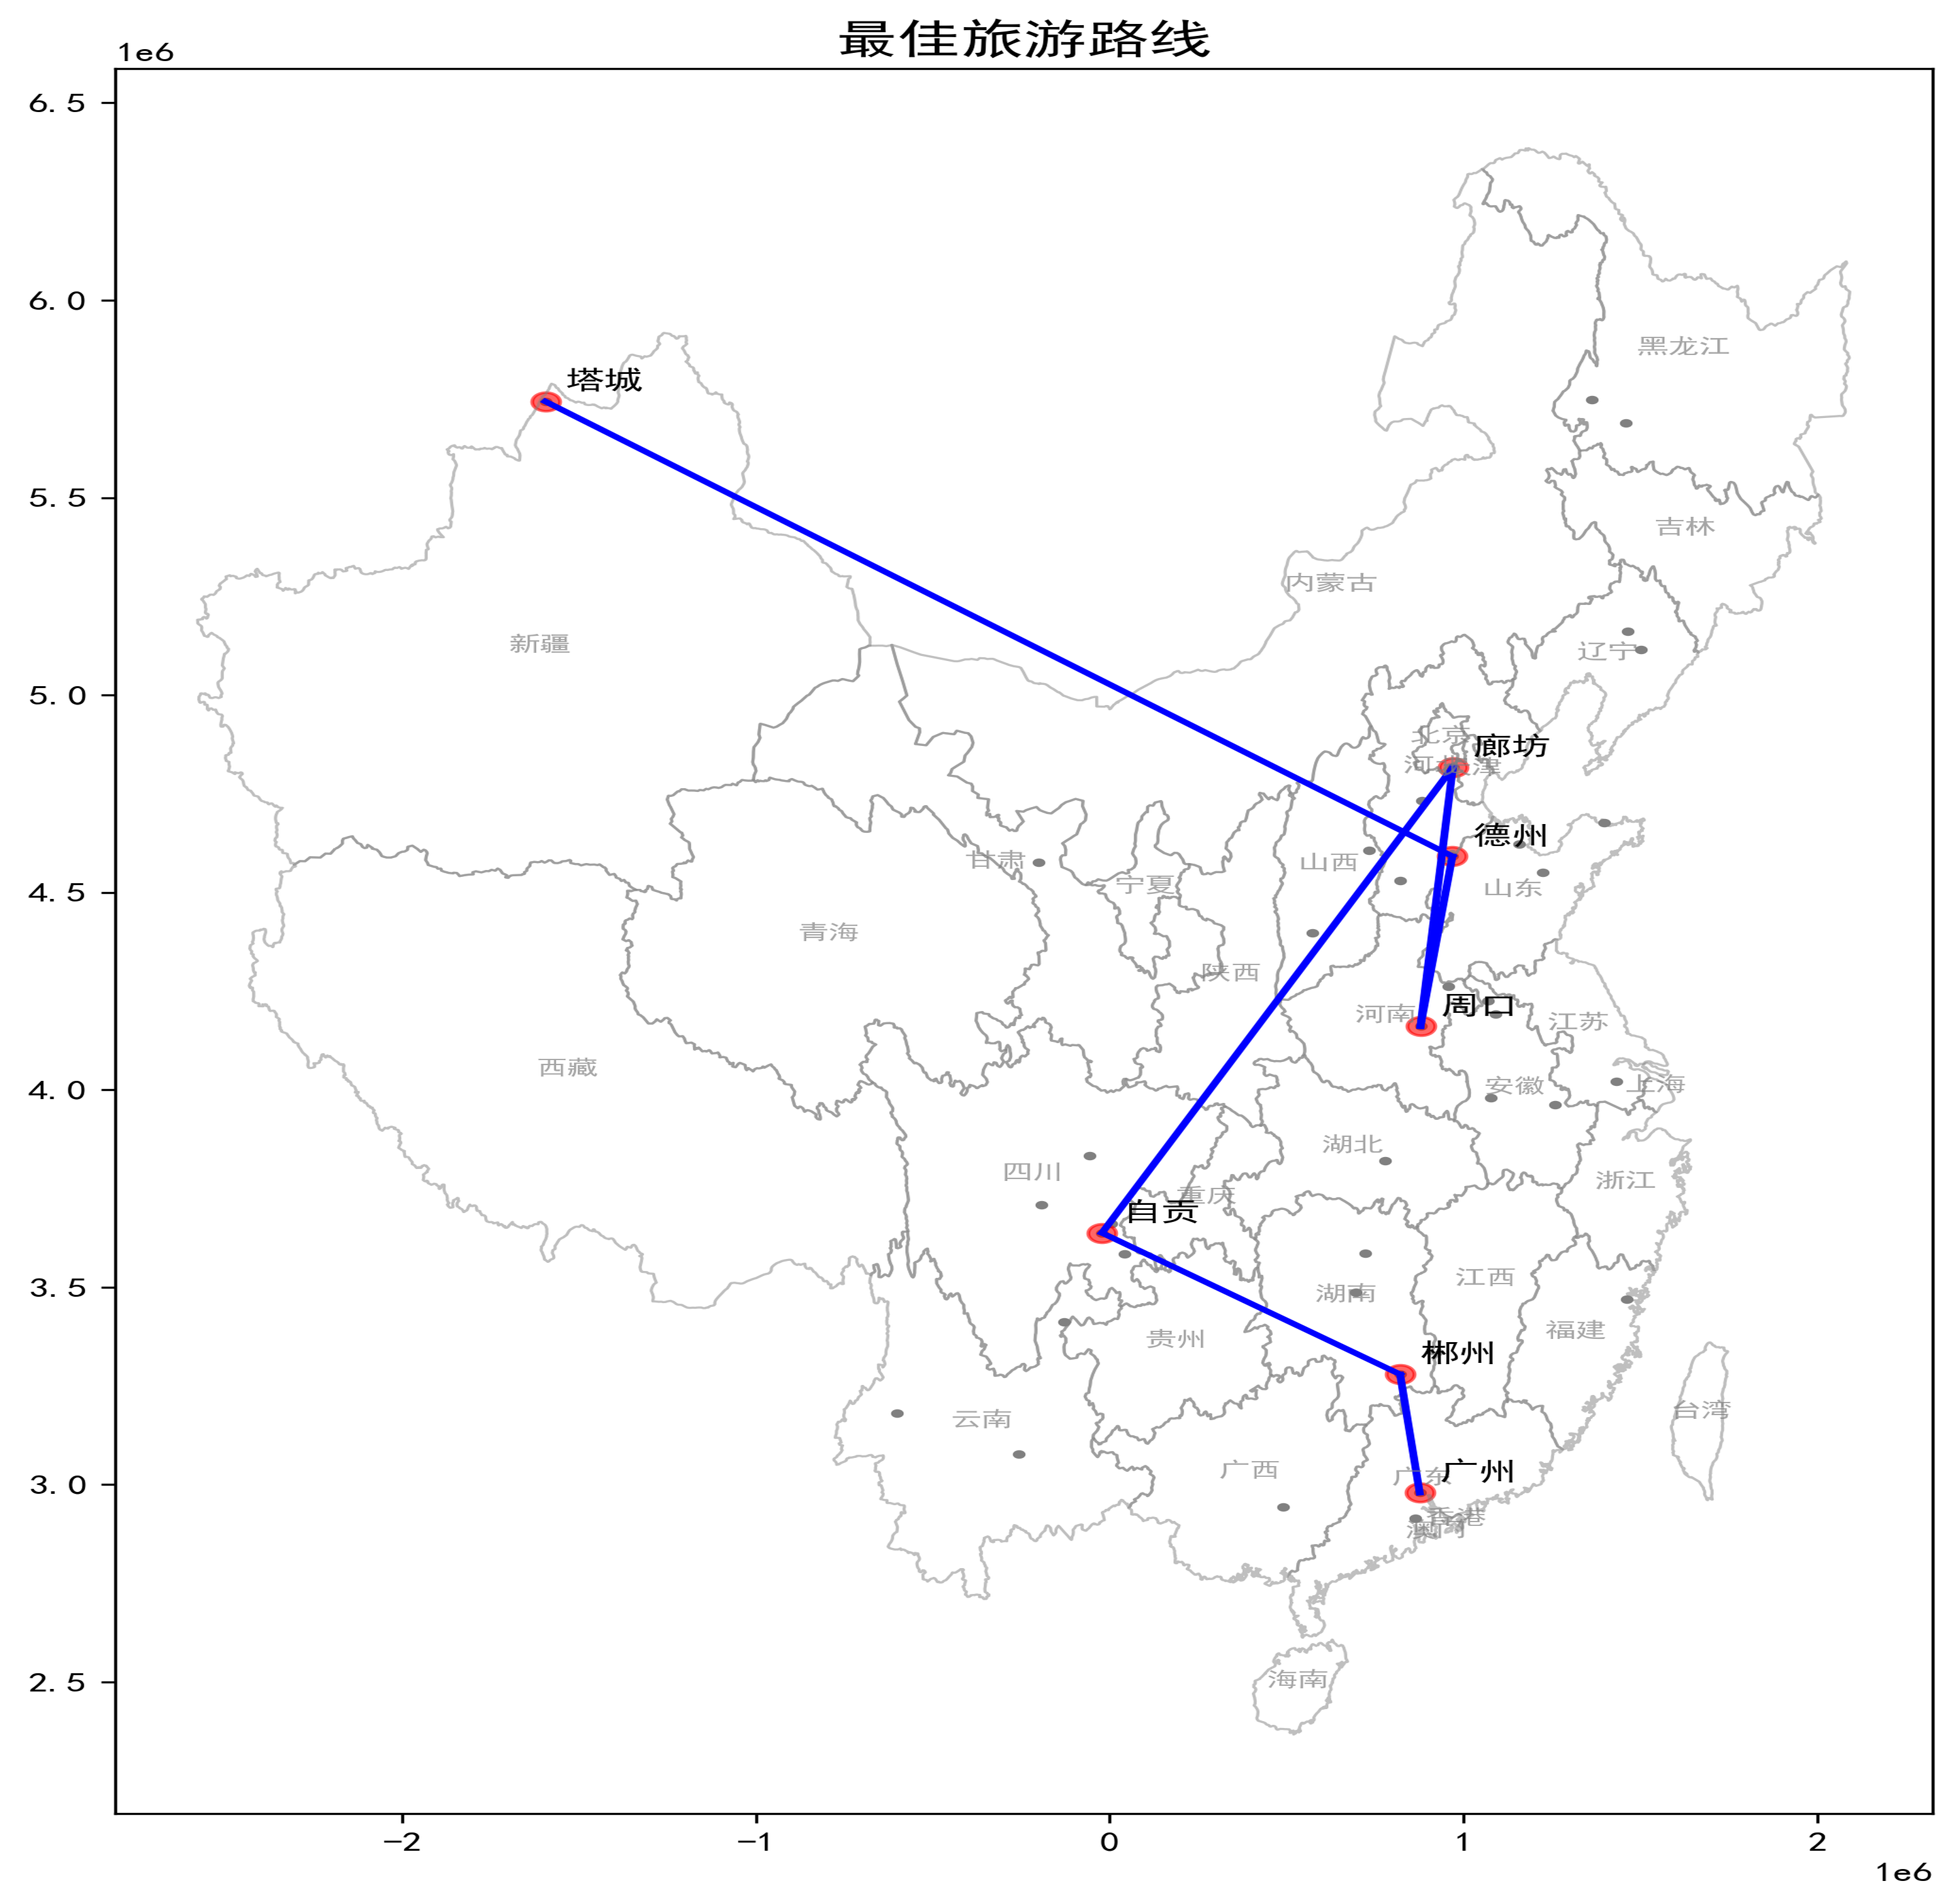
\includegraphics[width=1.0\textwidth]{figures/image/3_optimal_route.png}
    \caption{最佳旅游路线示意图}
    \label{fig:最佳旅游路线示意图}
\end{figure}

以广州为起点,
最优路线包括:广州→郴州→自贡→廊坊→周口→德州→塔城,
总计游览7个城市、62个景点,总时间约143.61小时,总费用约8353.29元。

%%%%%%%%%%%%%%%%%%%%%%%%%%%%%%%%%%%% 4.4 考虑经济因素的旅游路线优化模型 %%%%%%%%%%%%%%%%%%%%%%%%%%%%%%%%%%%%

\subsection{考虑经济因素的旅游路线优化模型}

\subsubsection{模型假设}
\begin{enumerate}
    \item 游客有预算限制,需要考虑交通费用和景点门票费用
    \item 高铁票价计算公式为:基础票价(20元) + 每公里费率(0.45元/公里) × 距离
    \item 景点门票费用与城市吸引力正相关
\end{enumerate}

\subsubsection{模型建立}
在前一个模型的基础上,我们引入经济因素,将问题重新定义为多目标优化问题:

\begin{equation}
\max \left\{ \sum_{c_i \in P} A(c_i), -\sum_{c_i \in P} C(c_i) - \sum_{j=1}^{k} F(c_{i_{j-1}}, c_{i_j}) \right\}
\end{equation}

其中$C(c_i)$为游览城市$c_i$的景点门票费用,$F(c_i, c_j)$为从城市$c_i$到城市$c_j$的交通费用,计算公式为:

\begin{equation}
F(c_i, c_j) = 20 + 0.45 \times D(c_i, c_j)
\end{equation}

为了平衡吸引力和费用,我们引入综合效用函数:

\begin{equation}
U(P) = \alpha \cdot \frac{\sum_{c_i \in P} A(c_i)}{A_{max}} - (1-\alpha) \cdot \frac{\sum_{c_i \in P} C(c_i) + \sum_{j=1}^{k} F(c_{i_{j-1}}, c_{i_j})}{C_{max}}
\end{equation}

其中$\alpha$为权重参数,$A_{max}$和$C_{max}$分别为最大可能的吸引力得分和费用。

\subsubsection{求解过程}
我们采用动态规划方法求解该多目标优化问题\cite{zhang2021}:

\begin{algorithm}[H]
    \renewcommand{\algorithmicrequire}{\textbf{Input:}}
	\renewcommand{\algorithmicensure}{\textbf{Output:}}
	\caption{Power method}
    \label{power}
    \begin{algorithmic}[1] % 控制是否有序号
\STATE 初始化状态数组$DP[i][t]$,表示游览前$i$个城市,用时$t$小时的最大效用
\FOR{$i = 1$ to $n$}
    \FOR{$t = 0$ to $144$}
        \FOR{$j = 0$ to $i-1$}
            \IF{$t \geq V(c_i) + T(c_j, c_i)$}
                \STATE $DP[i][t] = \max(DP[i][t], DP[j][t-V(c_i)-T(c_j, c_i)] + U(c_i))$
            \ENDIF
        \ENDFOR
    \ENDFOR
\ENDFOR
\end{algorithmic}
\end{algorithm}

\subsubsection{结果分析}
如表\ref{tab:最佳旅游路线规划(优化城市数量与费用)}、图\ref{fig:最佳旅游路线示意图(考虑费用因素与城市数量后)}所示,
考虑经济因素后,我们得到了一条更为经济实惠的旅游路线。

\begin{table}[H]
  \centering
  \caption{最佳旅游路线规划(优化城市数量与费用)}
  \label{tab:最佳旅游路线规划(优化城市数量与费用)}
  \begin{tabular}{|c|c|c|c|c|c|}
    \hline
    \textbf{城市} & \textbf{交通方式} & \textbf{交通时间(小时)} & \textbf{交通费用(元)} & \textbf{景点数量} & \textbf{门票费用(元)} \\
    \hline
    广州(起点) & - & - & - & 2 & 67 \\
    \hline
    郴州 & 高铁(从广州) & 6.0 & 694 & 8 & 200 \\
    \hline
    娄底 & 高铁(从郴州) & 10.1 & 1151 & 8 & 200 \\
    \hline
    塔城 & 高铁(从娄底) & 10.3 & 1174 & 8 & 15 \\
    \hline
    德州 & 高铁(从塔城) & 2.0 & 242 & 10 & 300 \\
    \hline
    无锡 & 高铁(从德州) & 5.4 & 629 & 8 & 200 \\
    \hline
    周口 & 高铁(从无锡) & 4.4 & 514 & 12 & 400 \\
    \hline
    淮北 & 高铁(从周口) & 10.5 & 1200 & 8 & 200 \\
    \hline
    保山 & 高铁(从淮北) & 10.2 & 1164 & 8 & 280 \\
    \hline
    \multicolumn{2}{|c|}{\textbf{总计}} & \textbf{58.9} & \textbf{6768} & \textbf{72} & \textbf{1862} \\
    \hline
    \multicolumn{5}{|c|}{\textbf{总游玩时间(小时)}} & \textbf{142.73} \\
    \hline
    \multicolumn{5}{|c|}{\textbf{总费用(元)}} & \textbf{8628.83} \\
    \hline
  \end{tabular}
\end{table}

\begin{figure}[H]
    \centering
    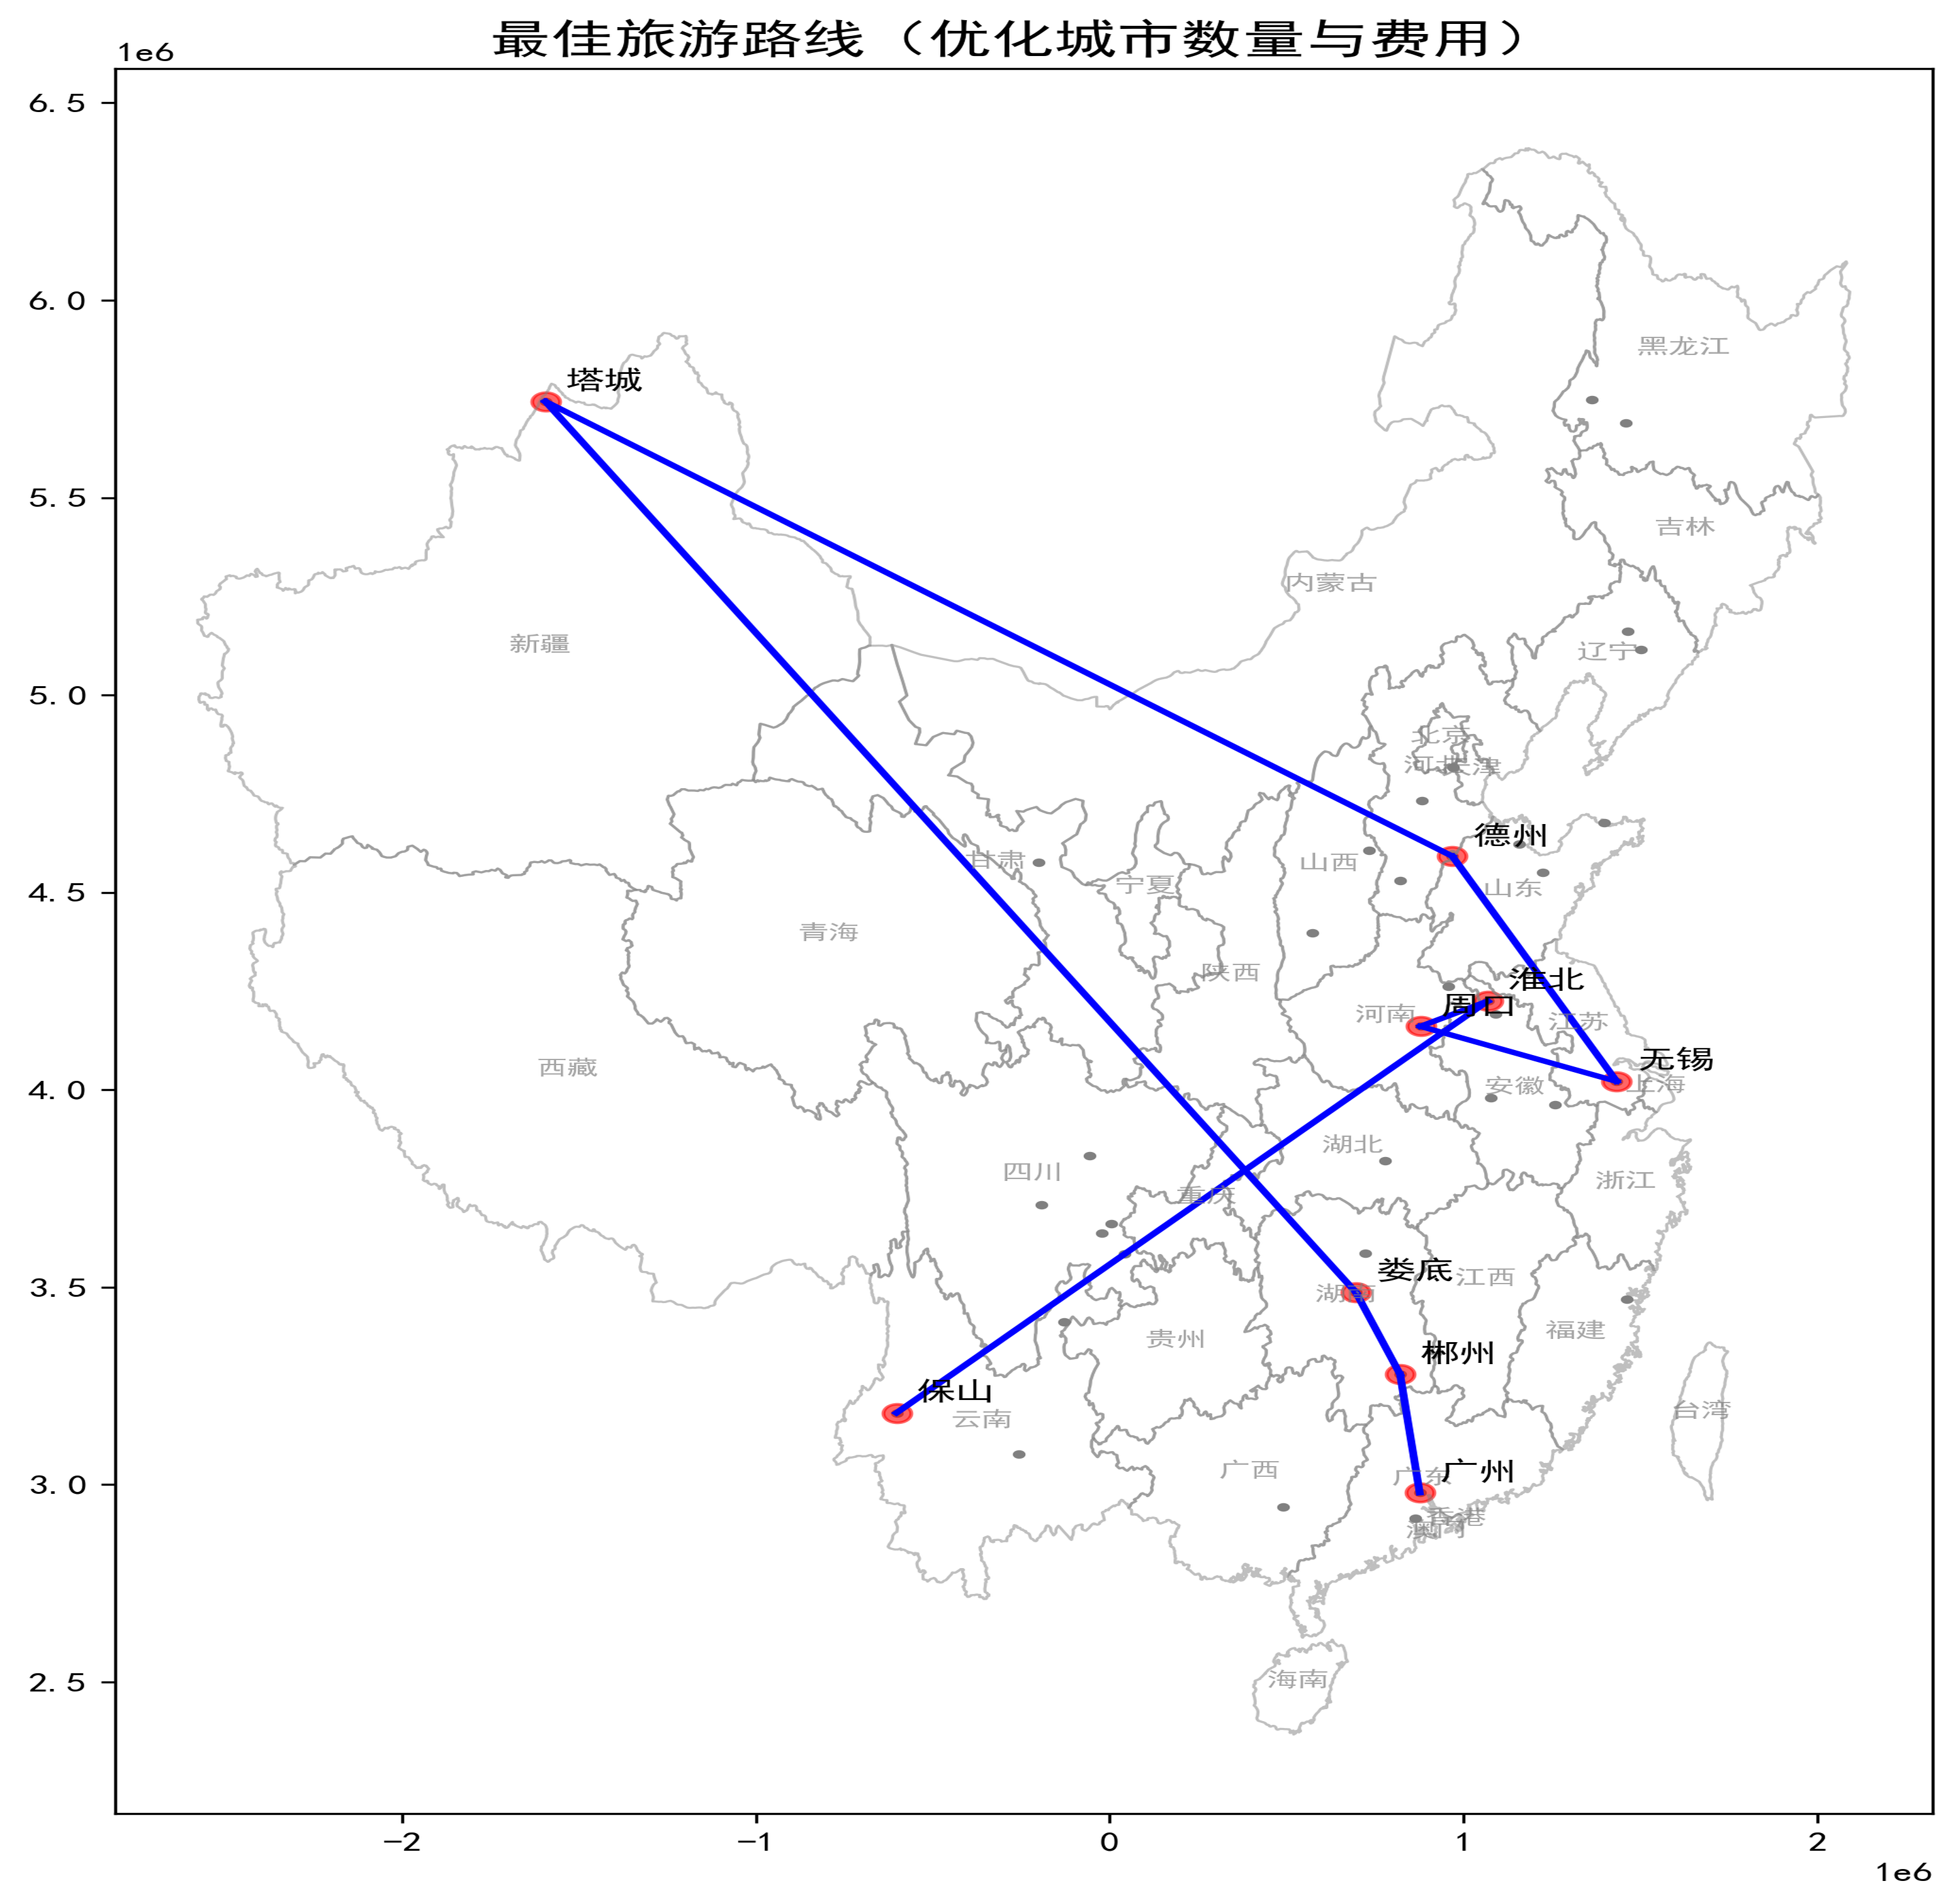
\includegraphics[width=1.0\textwidth]{figures/image/4_optimal_route.png}
    \caption{最佳旅游路线示意图(考虑费用因素与城市数量后)}
    \label{fig:最佳旅游路线示意图(考虑费用因素与城市数量后)}
\end{figure}

以广州为起点,考虑经济因素后优化后的路线包括:
广州→郴州→娄底→塔城→德州→无锡→周口→淮北→保山,总计游览9个城市、72个景点,
总时间约142.73小时,总费用约8628.83元。

虽然总费用略微上涨,但是游玩的景点数和城市数都明显增加。
原本游玩一个城市平均需要 8353.29 ÷ 7 ≈ 1193.33(元),游玩一个景点平均需要 8353.29 ÷ 62 ≈ 134.73(元);
现在游玩一个城市平均需要 8628.83 ÷ 9 ≈ 958.76(元),游玩一个景点平均需要 8628.83 ÷ 72 ≈ 119.84(元)。
可见考虑经济因素后的优化结果更加经济实惠,综合效用更高。






\subsection{山景旅游路线规划模型}

\subsubsection{模型假设}
\begin{enumerate}
    \item 外国游客对中国山景特别感兴趣
    \item 每个城市选择评分最高的山景景点进行游览
    \item 山景景点的游览时间与其评分正相关
\end{enumerate}

\subsubsection{模型建立}
我们首先筛选出含有山景景点的城市,然后为每个城市选择评分最高的山景景点。设山景景点集合为$M_i \subset A_i$,则城市$i$的最佳山景景点$m_i^*$为:

\begin{equation}
m_i^* = \arg\max_{j \in M_i} S_{ij}
\end{equation}

山景旅游路线规划问题可以建模为:

\begin{equation}
\max \sum_{c_i \in P} S(m_i^*)
\end{equation}

其中$S(m_i^*)$为城市$c_i$最佳山景景点的评分。

约束条件仍为总时间不超过144小时:

\begin{equation}
\sum_{c_i \in P} V(m_i^*) + \sum_{j=1}^{k} T(c_{i_{j-1}}, c_{i_j}) \leq 144
\end{equation}

其中$V(m_i^*)$为游览山景景点$m_i^*$所需的时间,根据评分确定:

\begin{equation}
V(m_i^*) = \begin{cases}
8, & \text{如果$S(m_i^*) \geq 4.5$} \\
6, & \text{如果$4.0 \leq S(m_i^*) < 4.5$} \\
4, & \text{如果$3.5 \leq S(m_i^*) < 4.0$} \\
3, & \text{其他情况}
\end{cases}
\end{equation}

\subsubsection{求解过程}
我们采用遗传算法求解该优化问题:

\begin{algorithm}[!ht]
    \renewcommand{\algorithmicrequire}{\textbf{Input:}}
	\renewcommand{\algorithmicensure}{\textbf{Output:}}
	\caption{Power method}
    \label{power}
    \begin{algorithmic}[1] % 控制是否有序号
\STATE 初始化种群,每个个体表示一条可行的旅游路线
\FOR{$g = 1$ to $G$}
    \STATE 计算每个个体的适应度(总评分)
    \STATE 选择适应度高的个体进行繁殖
    \STATE 对选中的个体进行交叉和变异
    \STATE 保留适应度最高的个体到下一代
\ENDFOR
\end{algorithmic}
\end{algorithm}

\subsubsection{结果分析}
如下列表\ref{tab:最佳山景旅游路线规划}、图\ref{fig:最佳山景旅游路线示意图}等所示,通过该模型,我们得到了一条专注于山景游览的最优路线。

\begin{table}[H]
  \centering
  \caption{最佳山景旅游路线规划}
  \label{tab:最佳山景旅游路线规划}
  \small % 或者 \footnotesize 更小
  \setlength{\tabcolsep}{4pt} % 减小列间距
  \begin{tabular}{|c|c|c|c|c|c|c|}
    \hline
    \textbf{序号} & \textbf{城市} & \textbf{景点名称} & \textbf{评分} & \textbf{交通方式} & \textbf{时间(h)} & \textbf{费用(元)} \\
    \hline
    1 & 北京 & 香山公园 & 4.7 & 入境城市 & - & - \\
    \hline
    2 & 淄博 & 傅山自然地质博物馆 & 5.0 & 高铁(从北京) & 0.7 & 94 \\
    \hline
    3 & 北海 & 鳄鱼山 & 4.6 & 高铁(从淄博) & 0.4 & 66 \\
    \hline
    4 & 信阳 & 金兰山 & 5.0 & 高铁(从北海) & 0.7 & 102 \\
    \hline
    5 & 阳江 & 大垌山净业寺 & 5.0 & 高铁(从信阳) & 1.0 & 132 \\
    \hline
    6 & 南阳 & 伏牛山地质公园 & 5.0 & 高铁(从阳江) & 0.9 & 122 \\
    \hline
    7 & 呼和浩特 & 圣水梁生态山庄 & 5.0 & 高铁(从南阳) & 3.1 & 364 \\
    \hline
    8 & 滁州 & 神山森林公园 & 5.0 & 高铁(从呼市) & 1.1 & 147 \\
    \hline
    9 & 娄底 & 大乘山 & 5.0 & 高铁(从滁州) & 4.5 & 527 \\
    \hline
    10 & 佳木斯 & 南山 & 5.0 & 高铁(从娄底) & 0.9 & 121 \\
    \hline
    11 & 榆林 & 白云山 & 4.5 & 高铁(从佳木斯) & 2.1 & 253 \\
    \hline
    12 & 黄山 & 黄山松 & 5.0 & 高铁(从榆林) & 2.1 & 256 \\
    \hline
    13 & 鹰潭 & 龙虎山仙宠乐园 & 4.1 & 高铁(从黄山) & 0.1 & 31 \\
    \hline
    14 & 孝感 & 应城国家矿山公园 & 4.3 & 高铁(从鹰潭) & 1.5 & 186 \\
    \hline
    15 & 杭州 & 超山赏梅 & 4.7 & 高铁(从孝感) & 3.4 & 402 \\
    \hline
    16 & 北京 & 香山公园 & 4.7 & 高铁(从杭州) & 5.0 & 583 \\
    \hline
  \end{tabular}
\end{table}


\begin{table}[H]
  \centering
  \caption{山景旅游路线游览信息}
  \label{tab:山景旅游路线游览信息}
  \begin{tabular}{|c|c|c|c|}
    \hline
    \textbf{序号} & \textbf{景点名称} & \textbf{游览时间(小时)} & \textbf{门票费用(元)} \\
    \hline
    1 & 香山公园 & 8 & 150 \\
    \hline
    2 & 淄博傅山自然地质博物馆 & 8 & 150 \\
    \hline
    3 & 鳄鱼山 & 8 & 150 \\
    \hline
    4 & 金兰山 & 8 & 150 \\
    \hline
    5 & 大垌山净业寺 & 8 & 150 \\
    \hline
    6 & 伏牛山地质公园 & 8 & 150 \\
    \hline
    7 & 圣水梁生态山庄 & 8 & 150 \\
    \hline
    8 & 神山森林公园 & 8 & 150 \\
    \hline
    9 & 大乘山 & 8 & 150 \\
    \hline
    10 & 南山 & 8 & 150 \\
    \hline
    11 & 白云山 & 8 & 150 \\
    \hline
    12 & 黄山松 & 8 & 150 \\
    \hline
    13 & 龙虎山仙宠乐园 & 6 & 120 \\
    \hline
    14 & 应城国家矿山公园 & 6 & 120 \\
    \hline
    15 & 超山赏梅 & 8 & 150 \\
    \hline
    16 & 香山公园 & 8 & 150 \\
    \hline
    \multicolumn{2}{|c|}{\textbf{总计}} & \textbf{124} & \textbf{2190} \\
    \hline
  \end{tabular}
\end{table}

\begin{table}[H]
  \centering
  \caption{山景旅游路线总结}
  \label{tab:山景旅游路线总结}
  \begin{tabular}{|c|c|}
    \hline
    \textbf{项目} & \textbf{数值} \\
    \hline
    总游玩时间 & 143.42小时 \\
    \hline
    总交通费用 & 3384.62元 \\
    \hline
    总门票费用 & 2190.00元 \\
    \hline
    总费用 & 5574.62元 \\
    \hline
    可游玩山景数量 & 16个 \\
    \hline
  \end{tabular}
\end{table}

\begin{figure}[H]
    \centering
    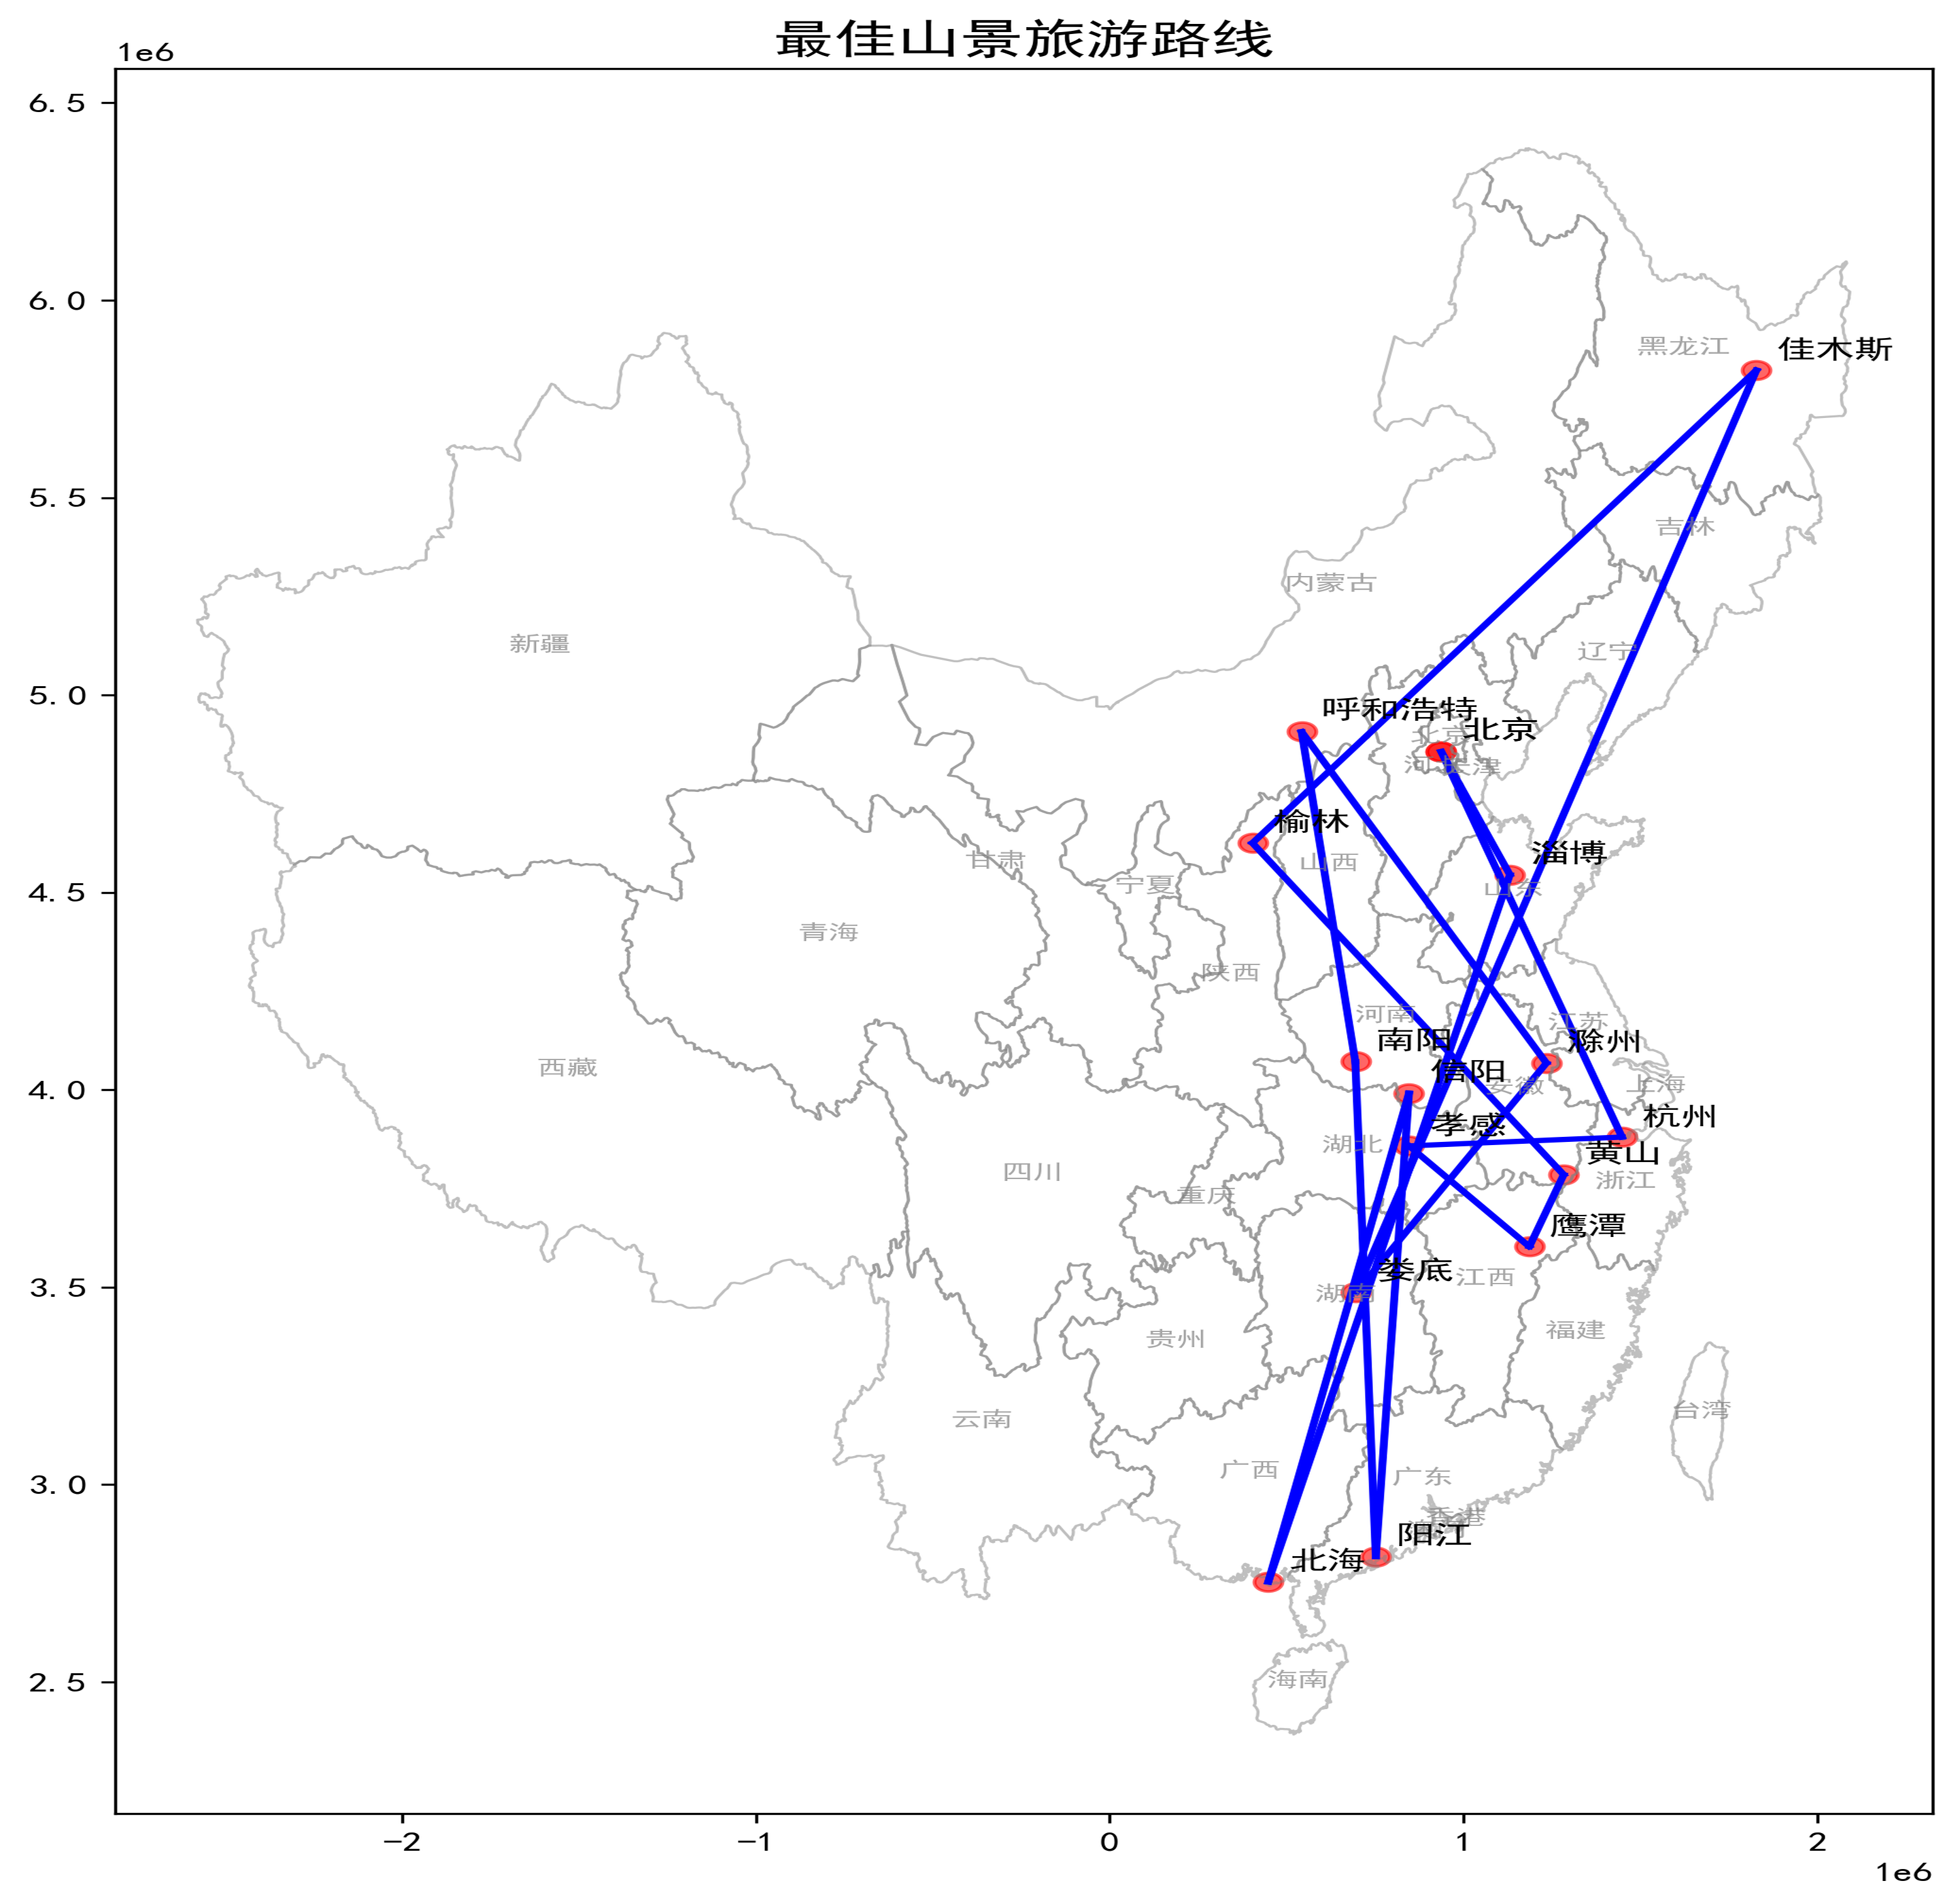
\includegraphics[width=1.0\textwidth]{figures/image/5.2_mountain_route.png}
    \caption{最佳山景旅游路线示意图}
    \label{fig:最佳山景旅游路线示意图}
\end{figure}

以北京为起点,最优路线包括:北京→淄博→北海→信阳→阳江→南阳→呼和浩特→滁州→娄底→佳木斯→榆林→黄山→鹰潭→孝感→杭州→北京,
总计游览16个城市的山景,总时间约143.42小时。
该路线的平均山景评分为4.7875,中间途径了北京香山公园、榆林白云山、黄山等山区景点,
为外国游客提供了一条高质量的中国山水风光之旅。





%%%%%%%%%%%%%%%%%%%%%%%%%%%%%%%%%%%%%%%%%%%%%%%%%%%%%%%%%%%% 5 模型评价 %%%%%%%%%%%%%%%%%%%%%%%%%%%%%%%%%%%%%%%%%%%%%%%%%%%%%%%%%%%%

\section{模型评价}

\subsection{模型优点}
\begin{enumerate}
    \item \textbf{多维数据整合能力}:本模型成功整合了景点评分、经典的地理位置、游览所需时间等多维数据,构建了一个全面的旅游价值评估体系,能够较为客观地反映城市和景点的实际吸引力。
    
    \item \textbf{层次化决策结构}:模型采用层次化的决策结构,先评估城市吸引力,再筛选最佳景点,最后规划旅游路线,使决策过程清晰有序,便于理解和实施。
    
    \item \textbf{时空约束的合理处理}:模型充分考虑了144小时的时间限制,将旅游时间、交通时间和景点游览时间进行了合理分配,确保规划的路线在现实中可行。
    
    \item \textbf{多目标优化能力}:在路线规划中,模型同时考虑了游览价值最大化和费用最小化两个目标,通过引入综合效用函数,实现了多目标的平衡优化。
    
    \item \textbf{个性化需求适应性}:模型能够根据不同游客的偏好(如山景爱好者)定制专属路线,体现了较强的个性化适应能力。
    
    \item \textbf{算法选择的合理性}:针对不同子问题,模型分别采用了贪心算法、动态规划和遗传算法等不同的求解方法,充分考虑了问题的特点和计算效率。
    
    \item \textbf{数据预处理的科学性}:模型对原始数据进行了系统的清洗和转换,特别是对景点评分和游览时间的标准化处理,提高了模型输入的质量。
\end{enumerate}

\subsection{模型局限性}
\begin{enumerate}
    \item \textbf{季节性因素的缺失}:模型未考虑季节变化对旅游体验的影响,如某些景点可能在特定季节更具吸引力(如春季赏花、秋季赏红叶),而在其他季节吸引力较低。这可能导致在不适宜的季节推荐某些景点。
    
    \item \textbf{交通方式的单一性}:模型假设城市间主要采用高铁交通,忽略了飞机、汽车、轮船等其他交通方式的可能性,以及不同交通方式之间的组合优化,这在某些区域(如西部山区、海岛等)可能不够实用。
    
    \item \textbf{景点拥挤度的忽略}:模型未考虑景点的实时拥挤程度和游客流量,而这些因素对旅游体验有显著影响。特别是在旅游旺季或节假日期间,热门景点可能过度拥挤,影响游览质量。
    
    \item \textbf{文化差异的简化处理}:虽然模型针对外国游客设计,但未深入考虑不同国家游客的文化背景差异和偏好差异,可能导致推荐的景点不符合特定文化背景游客的期望。
    
    \item \textbf{住宿因素的缺失}:模型主要关注景点游览和城市间交通,未将住宿选择和成本纳入考虑,而住宿是旅游规划的重要组成部分,会影响总体费用和体验。
    
    \item \textbf{天气条件的忽略}:未将天气因素纳入模型,而天气状况对户外景点的游览体验有显著影响。
    
    \item \textbf{模型验证的不足}:由于缺乏实际游客反馈数据,模型的有效性和准确性未能通过实际案例进行全面验证。
\end{enumerate}

\subsection{模型改进方向}
\begin{enumerate}
    \item \textbf{季节性动态调整机制}:引入季节性因素,建立景点吸引力的动态评估模型,针对不同季节提供差异化的路线推荐。可以收集各景点在不同季节的照片数量和评分变化,构建季节性吸引力指数。
    
    \item \textbf{多模式交通网络优化}:构建包含高铁、飞机、汽车、轮船等多种交通方式的综合交通网络模型,考虑不同交通方式的时间、费用、舒适度和可达性,实现最优交通组合方案。
    
    \item \textbf{实时客流量预测与控制}:整合景点实时游客流量数据,建立拥挤度预测模型,在路线规划中避开高峰期的热门景点,或调整游览顺序以优化体验。
    
    \item \textbf{文化背景个性化推荐}:基于不同国家游客的历史偏好数据,建立文化背景相似度模型,为来自不同国家的游客提供更符合其文化期望的个性化推荐。
    
    \item \textbf{住宿-景点联合优化}:将住宿选择纳入模型,考虑酒店位置、价格、评分等因素,实现住宿与景点游览的联合优化,减少不必要的往返时间。
    
    \item \textbf{天气敏感型路线规划}:引入天气预报数据,建立天气-景点适宜度评估模型,在不良天气条件下自动调整推荐室内景点,提高旅游体验的稳定性。
    
    \item \textbf{用户反馈学习机制}:设计用户反馈收集系统,通过实际游客的评价和建议不断优化模型参数和推荐算法,实现模型的自我学习和迭代改进。
    
    \item \textbf{语义分析与情感挖掘}:对景点评论进行深度语义分析和情感挖掘,提取更细粒度的景点特征和游客偏好信息,提高推荐的精准度。
    
    \item \textbf{可视化决策支持系统}:开发交互式可视化界面,允许用户根据自身偏好调整模型参数,实时查看不同路线方案的比较,增强用户参与度和决策透明度。
\end{enumerate}

通过以上评价和改进方向,我们可以看到,虽然当前模型在旅游路线规划方面取得了一定成果,但仍有较大的提升空间。未来工作将重点关注模型的动态适应性、个性化精准推荐以及实时优化能力,以期为外国游客提供更加完善、智能的中国旅游体验。


%%%%%%%%%%%%%%%%%%%%%%%%%%%%%%%%%%%%%%%%%%%%%%%%%%%%%%%%%%%% 6 模型推广 %%%%%%%%%%%%%%%%%%%%%%%%%%%%%%%%%%%%%%%%%%%%%%%%%%%%%%%%%%%%
\section{模型推广}

本文所建立的旅游路线规划模型具有较强的通用性和扩展性,可以推广应用到多种相关场景:

\subsection{国内游客旅游路线规划}
虽然本模型主要针对外国游客设计,但通过调整评价指标和权重,同样适用于国内游客:
\begin{enumerate}
    \item 针对不同地区游客的文化偏好,调整景点类型权重
    \item 考虑国内游客的消费习惯和时间安排特点
    \item 结合国内热门旅游季节和节假日人流量预测
\end{enumerate}

\subsection{特定主题旅游路线设计}
除了本文探讨的山景旅游路线外,模型可扩展到其他主题旅游:
\begin{enumerate}
    \item 历史文化之旅:重点关注博物馆、古迹、文化遗址等
    \item 美食之旅:结合各地特色美食和餐饮评分数据
    \item 自然生态之旅:关注国家公园、自然保护区等生态景观
    \item 红色旅游路线:针对革命历史遗址和纪念场所
\end{enumerate}

\subsection{多目的地综合旅游规划}
模型可扩展为多区域、跨国家的旅游规划工具:
\begin{enumerate}
    \item 亚洲多国联游路线规划,如"中日韩"或"东南亚+中国"组合
    \item 中国与"一带一路"沿线国家的跨境旅游路线
    \item 全球主要旅游城市的最优连接方案
\end{enumerate}

\subsection{智能旅游推荐系统}
将本模型与现代信息技术结合,开发智能旅游推荐系统:
\begin{enumerate}
    \item 结合用户画像和历史偏好,提供个性化旅游路线推荐
    \item 整合实时天气、交通、门票预约等数据,动态调整旅游计划
    \item 开发移动应用程序,提供实时导航和行程调整建议
    \item 引入增强现实(AR)技术,提升景点游览体验
\end{enumerate}

\subsection{城市规划与旅游资源开发}
本模型的分析方法可用于城市旅游资源评估与开发:
\begin{enumerate}
    \item 评估城市旅游资源分布与开发潜力
    \item 为旅游基础设施建设提供决策支持
    \item 优化城市间交通网络,提高旅游可达性
    \item 发掘潜在旅游热点,促进区域均衡发展
\end{enumerate}

\subsection{旅游大数据分析平台}
将模型扩展为综合性旅游大数据分析平台:
\begin{enumerate}
    \item 整合多源旅游数据,包括评论、照片、视频等用户生成内容
    \item 分析旅游流量模式和游客行为特征
    \item 预测旅游热点变化趋势和市场需求
    \item 为旅游管理部门和企业提供决策支持
\end{enumerate}

通过以上推广应用,本文所建立的旅游路线规划模型可以在更广泛的领域发挥作用,为旅游业的智能化、个性化发展提供理论支持和实践指导。同时,随着大数据、人工智能等技术的不断发展,模型的精确性和适用性也将进一步提升,为游客提供更加优质的旅游体验。

\newpage % 分页符

%%%%%%%%%%%%%%%%%%%%%%%%%%%%%%%%%%%%%%%%%%%%%%%%%%%%%%%%%%%% 参考文献 %%%%%%%%%%%%%%%%%%%%%%%%%%%%%%%%%%%%%%%%%%%%%%%%%%%%%%%%%%%%

% \cite{liuhaiyang2013latex}

\begin{thebibliography}{9}%宽度9

    \bibitem{shanghai2013}
    上海2013年1月起对45国开放72小时过境免签\allowbreak[J].
    \newblock 空运商务, 2012(23):29-29.

    \bibitem{sun2024}
    Sun, F.; Li, Z.; Xu, M.; Han, M. New Changes in Chinese Urban Tourism Pattern under the Impact of COVID-19 Pandemic: Based on Internet Attention\allowbreak[J].
    \newblock Sustainability, 2024, 16(14):5853.

    \bibitem{lan2017}
    蓝兰. 我国高铁运营里程超两万公里完全自主化加速推进\allowbreak[J].
    \newblock 交通建设与管理, 2017(4):56-61.

    \bibitem{li2021}
    Li, Y.; Gan, H. Tourism Information Data Processing Method Based on Multi-Source Data Fusion\allowbreak[J].
    \newblock Journal of Sensors, 2021. https://doi.org/10.1155/2021/7047119


    \bibitem{kariam2022}
    Kariam, W. S.; Setyabudi, I. Persepsi Akademisi Bidang Lanskap Terhadap Objek Wisata Coban Talun di Kota Batu\allowbreak[J].
    \newblock TRANSFORM: Journal of Tropical Architecture and Sustainable Urban Science, 2022, 1(2):89-93. https://doi.org/10.30872/transform.v1i2.115


    \bibitem{profillidis2013}
    Profillidis, V.; Botzoris, G. High-Speed Railways: Present Situation and Future Prospects\allowbreak[J].
    \newblock Journal of Transportation Technologies, 2013, 3(2A):30-36. doi: 10.4236/jtts.2013.32A004.

    \bibitem{colson1914}
    Colson, C.; Christie, L. R.; Leedam, G.; Travis, C. Railway Rates and Traffic\allowbreak[M].
    \newblock London: G. Bell and Sons, Ltd., 1914.

    \bibitem{xiang2022}
    Xiang, D.; Lin, H.; Ouyang, J. et al. Combined improved A* and greedy algorithm for path planning of multi-objective mobile robot\allowbreak[J].
    \newblock Scientific Reports, 2022, 12:13273. https://doi.org/10.1038/s41598-022-17684-0

    \bibitem{zhang2021}
    张皓然; 孙冬璞; 季发虎; 等. 基于动态规划策略的旅游路线规划\allowbreak[J].
    \newblock 计算机与数字工程, 2021, 49(2):301-304,346. DOI:10.3969/j.issn.1672-9722.2021.02.015.

    \bibitem{moraes2013}
    Moraes, W.; Ribeiro, G.; Emmendoerfer, M. Ensaio de uma metodologia com indicadores para o turismo de base comunitária: O caso do Território da Serra do Brigadeiro - Brasil\allowbreak[J].
    \newblock PASOS Revista de turismo y patrimonio cultural, 2013, 11:297-312. DOI:10.25145/j.pasos.2013.11.019.


\end{thebibliography}





\newpage % 分页符

%%%%%%%%%%%%%%%%%%%%%%%%%%%%%%%%%%%%%%%%%%%%%%%%%%%%%%%%%%%% 附录 %%%%%%%%%%%%%%%%%%%%%%%%%%%%%%%%%%%%%%%%%%%%%%%%%%%%%%%%%%%%
\begin{appendices}

%%%%%%%%%%%%%%%%%%%%%%%%%%%%%%%%%%%% 附录A 文件列表 %%%%%%%%%%%%%%%%%%%%%%%%%%%%%%%%%%%%%
\section{文件列表}

本项目包含以下文件:

\begin{table}[H]
\centering
\caption{项目文件列表}
\label{tab:file_list}
\begin{tabular}{|p{5cm}|p{10cm}|}
\hline
\textbf{文件名} & \textbf{描述} \\
\hline
1.py & 用于分析城市景点评分数据,计算最高评分及其分布情况 \\
\hline
2.1.py & 提取每个城市最高评分景点数据并保存到独立文件 \\
\hline
2.2.py & 基于景点评分和数量计算城市吸引力,评选最受外国游客向往的50个城市 \\
\hline
3.py & 基于贪心算法的旅游路线规划模型,从广州出发规划144小时旅游路线 \\
\hline
4.py & 考虑经济因素的旅游路线优化模型,平衡景点数量与旅游成本 \\
\hline
5.1.py & 筛选各城市中名称包含"山"字的景点,提取山景相关数据 \\
\hline
5.2.py & 基于遗传算法的山景旅游路线规划模型,为山景爱好者定制路线 \\
\hline
data/ & 包含352个城市的景点数据文件夹,每个城市一个CSV文件 \\
\hline
2.1\_best\_attractions/ & 存储每个城市最高评分景点的输出文件夹 \\
\hline
5.1\_filtered\_mountain\_data/ & 存储筛选后的山景景点数据的输出文件夹 \\
\hline
3\_地级城市驻地.geojson & 中国地级市地理位置数据,用于路线规划和可视化 \\
\hline
3\_省级行政区.geojson & 中国省级行政区边界数据,用于地图背景绘制 \\
\hline
figures/image/ & 存储生成的路线规划图像和其他可视化结果 \\
\hline
\end{tabular}
\end{table}

\subsection{数据文件说明}

每个城市的景点数据CSV文件包含以下字段:
\begin{itemize}
    \item \textbf{名字}:景点名称
    \item \textbf{评分}:景点评分(0-5分)
    \item \textbf{评论数}:游客评论数量
    \item \textbf{类型}:景点类型(如自然风光、历史古迹等)
    \item \textbf{地址}:景点详细地址
    \item \textbf{建议游玩时间}:推荐的游览时长
    \item \textbf{门票}:景点门票价格信息
\end{itemize}

\subsection{输出文件说明}

模型运行后生成以下输出文件:
\begin{itemize}
    \item \textbf{1\_res.txt}:问题1的分析结果,包含最高评分及其分布情况
    \item \textbf{2.2\_top\_50\_cities\_for\_foreign\_tourists.csv}:最受外国游客向往的50个城市列表
    \item \textbf{3\_optimal\_route.png}:从广州出发的最佳旅游路线可视化图
    \item \textbf{3\_travel\_route\_report.html}:问题3的详细旅游路线报告
    \item \textbf{4\_optimal\_route.png}:考虑经济因素后的优化旅游路线可视化图
    \item \textbf{4\_travel\_route\_report.html}:问题4的详细旅游路线报告
    \item \textbf{5.2\_mountain\_route.png}:山景旅游路线可视化图
    \item \textbf{5.2\_mountain\_route\_report.html}:问题5的山景旅游路线详细报告
\end{itemize}

\subsection{环境依赖}

本项目的Python代码依赖以下库:
\begin{itemize}
    \item \textbf{pandas}:数据处理与分析
    \item \textbf{numpy}:数值计算
    \item \textbf{matplotlib}:数据可视化
    \item \textbf{geopandas}:地理数据处理
    \item \textbf{networkx}:网络图构建与分析
    \item \textbf{pyproj}:坐标系转换
\end{itemize}




%%%%%%%%%%%%%%%%%%%%%%%%%%%%%%%%%%%% 附录B 代码 %%%%%%%%%%%%%%%%%%%%%%%%%%%%%%%%%%%%%

\section{代码}

\textbf{1.py}
\begin{lstlisting}[language=python]
import os
import pandas as pd
import numpy as np
from collections import Counter

# 设置数据文件夹路径
data_folder = 'data'

# 存储所有城市的景点评分数据
all_scores = []
# 存储每个城市拥有最高分景点的数量
city_bs_count = {}

# 遍历所有城市文件
for city_file in os.listdir(data_folder):
    if city_file.endswith('.csv'):
        city_name = city_file[:-4]  # 去掉.csv后缀得到城市名
        file_path = os.path.join(data_folder, city_file)
        
        try:
            # 读取CSV文件,指定编码为utf-8
            df = pd.read_csv(file_path, encoding='utf-8')
            
            # 提取评分列,处理非数字值
            scores = []
            for score in df['评分']:
                try:
                    if score and score != '--':  # 检查是否为空或'--'
                        scores.append(float(score))
                except:
                    # 忽略无法转换为浮点数的值
                    pass
            
            # 添加到所有评分列表
            all_scores.extend(scores)
            
            # 记录城市信息,用于后续统计
            city_bs_count[city_name] = 0
            
        except Exception as e:
            print(f"处理文件 {city_file} 时出错: {e}")

# 计算最高评分(BS)
best_score = max(all_scores) if all_scores else 0
print(f"问题1-1: 最高评分(BS)是: {best_score}")

# 统计获得最高评分的景点数量
bs_count = all_scores.count(best_score)
print(f"问题1-2: 全国有 {bs_count} 个景点获评最高评分(BS)")

# 重新遍历所有城市文件,统计每个城市拥有最高评分景点的数量
for city_file in os.listdir(data_folder):
    if city_file.endswith('.csv'):
        city_name = city_file[:-4]
        file_path = os.path.join(data_folder, city_file)
        
        try:
            df = pd.read_csv(file_path, encoding='utf-8')
            
            # 统计该城市拥有最高评分的景点数量
            bs_count_city = 0
            for score in df['评分']:
                try:
                    if score and score != '--' and float(score) == best_score:
                        bs_count_city += 1
                except:
                    pass
            
            city_bs_count[city_name] = bs_count_city
            
        except Exception as e:
            print(f"处理文件 {city_file} 时出错: {e}")

# 按照拥有最高评分景点数量排序城市
sorted_cities = sorted(city_bs_count.items(), key=lambda x: x[1], reverse=True)

# 获得拥有最高评分景点最多的城市(可能有多个并列)
max_bs_count = sorted_cities[0][1]
top_cities = [city for city, count in sorted_cities if count == max_bs_count]

print(f"问题1-3: 获评最高评分(BS)景点最多的城市是: {', '.join(top_cities)}, 各有 {max_bs_count} 个最高评分景点")

# 列出前10个拥有最高评分景点数量最多的城市
print("问题1-4: 依据拥有最高评分景点数量排序,前10个城市是:")
for i, (city, count) in enumerate(sorted_cities[:10], 1):
    print(f"{i}. {city}: {count}个最高评分景点")

# 将结果输出到文件
with open('1_res.txt', 'w', encoding='utf-8') as f:
    f.write(f"问题1-1: 最高评分(BS)是: {best_score}\n")
    f.write(f"问题1-2: 全国有 {bs_count} 个景点获评最高评分(BS)\n")
    f.write(f"问题1-3: 获评最高评分(BS)景点最多的城市是: {', '.join(top_cities)}, 各有 {max_bs_count} 个最高评分景点\n")
    f.write("问题1-4: 依据拥有最高评分景点数量排序,前10个城市是:\n")
    for i, (city, count) in enumerate(sorted_cities[:10], 1):
        f.write(f"{i}. {city}: {count}个最高评分景点\n")
 \end{lstlisting}


\textbf{2.1.py}
\begin{lstlisting}[language=python]
import os
import pandas as pd
import numpy as np
import csv
import warnings
warnings.filterwarnings('ignore')

# 创建输出文件夹(如果不存在)
output_folder = '2.1_best_attractions'
if not os.path.exists(output_folder):
    os.makedirs(output_folder)

# 读取data文件夹下的所有csv文件
data_folder = 'data'
city_files = [f for f in os.listdir(data_folder) if f.endswith('.csv')]

for city_file in city_files:
    try:
        # 读取城市CSV文件
        city_name = city_file.split('.')[0]
        file_path = os.path.join(data_folder, city_file)
        
        # 使用pandas读取CSV文件,指定编码为utf-8
        df = pd.read_csv(file_path, encoding='utf-8')
        
        # 将评分列转换为数值类型,非数值记为NaN
        df['评分'] = pd.to_numeric(df['评分'], errors='coerce')
        
        # 找出该城市的最高评分
        max_score = df['评分'].max()
        
        # 筛选出评分等于最高评分的景点
        best_attractions = df[df['评分'] == max_score]
        
        # 保存到输出文件夹中的同名CSV文件
        output_path = os.path.join(output_folder, city_file)
        best_attractions.to_csv(output_path, index=False, encoding='utf-8')
        
        print(f"已处理 {city_name},最高评分: {max_score},共有 {len(best_attractions)} 个最高评分景点")
    
    except Exception as e:
        print(f"处理 {city_file} 时出错: {str(e)}")

print("所有城市处理完成!")

 \end{lstlisting}




 \textbf{2.2.py}
\begin{lstlisting}[language=python]
import os
import pandas as pd
import glob
import re

def extract_hours(time_str):
    """Extract hours from the suggested visiting time string"""
    if pd.isna(time_str):
        return 24  # Default to 24 hours if no time is specified
    
    time_str = str(time_str).lower()
    
    # Handle different time formats
    if '小时' in time_str:
        # Extract numeric values
        numbers = re.findall(r'\d+\.?\d*', time_str)
        if numbers:
            if '-' in time_str:  # Range like "0.5小时 - 1小时"
                return (float(numbers[0]) + float(numbers[1])) / 2
            else:  # Single value like "2小时"
                return float(numbers[0])
    
    elif '天' in time_str:
        numbers = re.findall(r'\d+\.?\d*', time_str)
        if numbers:
            if '-' in time_str:  # Range like "1天 - 3天"
                return (float(numbers[0]) + float(numbers[1])) / 2 * 24
            else:  # Single value like "3天"
                return float(numbers[0]) * 24
    
    return 24  # Default value if parsing fails

def get_best_attractions():
    """Read all CSV files in the best_attractions folder and process them"""
    csv_files = glob.glob('2.1_best_attractions/*.csv')
    city_best_attractions = []
    
    for file_path in csv_files:
        city_name = os.path.basename(file_path).replace('.csv', '')
        
        try:
            df = pd.read_csv(file_path)
            if df.empty:
                continue
            
            # Calculate the number of best attractions for this city
            best_attractions_count = len(df)
            
            # Get the first attraction (we'll process all and calculate a weighted score)
            attraction_info = df.iloc[0].to_dict()
            
            # Extract and process suggested visiting time
            suggested_time = extract_hours(attraction_info.get('建议游玩时间', 24))
            
            # Normalize the visiting time score (shorter time is better)
            time_score = 1 / (1 + suggested_time)  # Add 1 to avoid division by zero
            
            # Calculate a weighted score (rating 60%, count 30%, time 10%)
            rating = float(attraction_info.get('评分', 0))
            weighted_score = 0.6 * rating + 0.3 * best_attractions_count + 0.1 * time_score * 10
            
            # Add additional information
            attraction_info['城市'] = city_name
            attraction_info['最佳景点数量'] = best_attractions_count
            attraction_info['建议游玩小时数'] = suggested_time
            attraction_info['加权评分'] = weighted_score
            
            # Ensure rating is float
            attraction_info['评分'] = float(attraction_info.get('评分', 0))
            
            city_best_attractions.append(attraction_info)
            
        except Exception as e:
            print(f"处理文件 {file_path} 时出错: {e}")
    
    return city_best_attractions

def main():
    # Get all city attractions with processed information
    city_attractions = get_best_attractions()
    
    # Create DataFrame
    df = pd.DataFrame(city_attractions)
    
    # Sort by weighted score (descending), then by rating (descending), then by count (descending)
    df_sorted = df.sort_values(
        by=['加权评分', '评分', '最佳景点数量'], 
        ascending=[False, False, False]
    )
    
    # Select top 50 cities
    top_50_cities = df_sorted.head(50)
    
    # Output results
    print("最令外国游客向往的50个城市:")
    for i, (index, row) in enumerate(top_50_cities.iterrows(), 1):
        print(f"{i}. {row['城市']} - 最佳景点: {row['名字']}, 评分: {row['评分']:.1f}, "
              f"最佳景点数量: {row['最佳景点数量']}, 建议游玩小时数: {row['建议游玩小时数']:.1f}")
    
    # Save results
    top_50_cities.to_csv('2.2_top_50_cities_for_foreign_tourists.csv', index=False)
    print("结果已保存到 2.2_top_50_cities_for_foreign_tourists.csv")

if __name__ == "__main__":
    main()
 \end{lstlisting}





 \textbf{3.py}
\begin{lstlisting}[language=python]
import pandas as pd
import numpy as np
import geopandas as gpd
from math import radians, cos, sin, asin, sqrt
import networkx as nx
import matplotlib.pyplot as plt
from pyproj import Transformer
import matplotlib as mpl
from matplotlib.font_manager import FontProperties
import webbrowser
import os

# 解决中文显示问题
plt.rcParams['font.sans-serif'] = ['SimHei']  # 使用黑体 [[0]](#__0)
plt.rcParams['axes.unicode_minus'] = False    # 解决负号显示问题 [[1]](#__1)

# 1. 加载数据
def load_data():
    # 加载最令外国游客向往的50个城市数据
    top_cities = pd.read_csv('2.2_top_50_cities_for_foreign_tourists.csv')
    
    # 加载城市地理位置数据
    city_locations = gpd.read_file('3_地级城市驻地.geojson')
    
    # 加载省级行政区数据
    provinces = gpd.read_file('3_省级行政区.geojson')
    
    # 加载广州景点数据
    guangzhou_attractions = pd.read_csv('2.1_best_attractions/广州.csv')
    
    return top_cities, city_locations, provinces, guangzhou_attractions
# 2. 计算两个城市之间的距离

def calculate_distance(x1, y1, x2, y2):
    """
    使用Haversine公式计算两个坐标点之间的距离(单位:公里)
    """
    # 将经纬度转换为弧度
    lon1, lat1, lon2, lat2 = map(radians, [x1, y1, x2, y2])
    
    # Haversine公式
    dlon = lon2 - lon1
    dlat = lat2 - lat1
    a = sin(dlat/2)**2 + cos(lat1) * cos(lat2) * sin(dlon/2)**2
    c = 2 * asin(sqrt(a))
    r = 6371  # 地球平均半径,单位为公里
    
    return c * r

# 3. 估算高铁交通时间和费用
def estimate_travel_time_and_cost(distance):
    """
    根据距离估算高铁交通时间(小时)和费用(元)
    """
    # 假设高铁平均速度为250km/h 
    travel_time = distance / 250
    
    # 高铁票价估算公式: 基础票价 + 每公里费率 
    base_fare = 20
    rate_per_km = 0.45
    travel_cost = base_fare + distance * rate_per_km
    
    return travel_time, travel_cost

# 4. 计算城市的吸引力得分
def calculate_city_attraction_score(city_row, top_cities_df):
    """
    计算城市的吸引力得分
    """
    city_name = city_row['name']
    
    # 检查城市是否在top_cities中
    if city_name in top_cities_df['城市'].values:
        # 假设top_cities_df中有排名信息,排名越高分数越高
        rank = top_cities_df[top_cities_df['城市'] == city_name].index[0] + 1
        # 排名越低,分数越高(反向关系)
        attraction_score = 51 - rank  # 假设共50个城市,排名第1的得分为50
    else:
        attraction_score = 0  # 不在列表中的城市吸引力为0
    
    return attraction_score

# 5. 估算每个城市的游览时间
def estimate_visit_time(city_name, top_cities_df):
    """
    估算游览一个城市所需的时间(小时)
    """
    # 根据城市在列表中的排名来确定游览时间
    if city_name in top_cities_df['城市'].values:
        rank = top_cities_df[top_cities_df['城市'] == city_name].index[0] + 1
        
        # 排名越高的城市,游览时间越长(更多景点)
        if rank <= 10:
            visit_time = 24  # 一线城市需要一整天
        elif rank <= 20:
            visit_time = 18  # 二线城市需要18小时
        elif rank <= 30:
            visit_time = 12  # 三线城市需要12小时
        else:
            visit_time = 8   # 其他城市需要8小时
    else:
        visit_time = 6  # 不在列表中的城市默认6小时
    
    return visit_time

# 6. 规划最佳旅游路线
def plan_optimal_route(top_cities, city_locations, guangzhou_attractions, start_city="广州", max_hours=144):
    """
    规划最佳旅游路线
    """
    # 检查广州是否在城市位置数据中
    if start_city not in city_locations['name'].values:
        raise ValueError(f"起始城市 {start_city} 不在地理位置数据中")
    
    # 为广州添加一个较高的吸引力分数,确保它被包含在路线中
    if start_city not in top_cities['城市'].values:
        print(f"警告: 起始城市 {start_city} 不在最令外国游客向往的50个城市列表中")
    
    # 创建城市图
    G = nx.Graph()
    
    # 添加节点(所有在top_cities中的城市以及起始城市)
    valid_cities = []
    for idx, city in city_locations.iterrows():
        city_name = city['name']
        
        # 如果是起始城市或在top_cities中,则添加到图中
        if city_name == start_city or city_name in top_cities['城市'].values:
            # 计算吸引力得分和游览时间
            attraction_score = calculate_city_attraction_score(city, top_cities)
            visit_time = estimate_visit_time(city_name, top_cities)
            
            # 添加节点
            G.add_node(city_name, 
                      x=city.geometry.x, 
                      y=city.geometry.y, 
                      attraction_score=attraction_score,
                      visit_time=visit_time)
            valid_cities.append(city_name)
    
    # 添加边(城市之间的连接)
    for i in range(len(valid_cities)):
        for j in range(i+1, len(valid_cities)):
            city1 = valid_cities[i]
            city2 = valid_cities[j]
            
            # 计算距离
            x1, y1 = G.nodes[city1]['x'], G.nodes[city1]['y']
            x2, y2 = G.nodes[city2]['x'], G.nodes[city2]['y']
            distance = calculate_distance(x1, y1, x2, y2)
            
            # 估算交通时间和费用
            travel_time, travel_cost = estimate_travel_time_and_cost(distance)
            
            # 添加边
            G.add_edge(city1, city2, distance=distance, travel_time=travel_time, travel_cost=travel_cost)
    
    # 寻找最佳路线
    # 使用贪婪算法: 从起始城市开始,每次选择能够最大化体验/时间比的下一个城市
    current_city = start_city
    route = [current_city]
    total_time = G.nodes[current_city]['visit_time']  # 初始城市游览时间
    
    # 获取门票价格
    if current_city == "广州":
        ticket_price = calculate_guangzhou_ticket_price(guangzhou_attractions)
    else:
        ticket_price = parse_ticket_price(
            top_cities[top_cities['城市'] == current_city]['门票'].values[0] if current_city in top_cities['城市'].values else None,
            top_cities, current_city
        )
        
    total_cost = ticket_price  # 初始城市费用包含门票
    total_attractions = 0
    
    # 已访问城市集合
    visited = {current_city}
    
    while total_time < max_hours:
        best_next_city = None
        best_score = -1
        
        # 遍历所有相邻城市
        for neighbor in valid_cities:
            if neighbor in visited:
                continue
                
            # 计算到达该城市的交通时间和费用
            travel_time = G[current_city][neighbor]['travel_time']
            travel_cost = G[current_city][neighbor]['travel_cost']
            
            # 游览该城市所需时间
            visit_time = G.nodes[neighbor]['visit_time']
            
            # 检查是否超出总时间限制
            if total_time + travel_time + visit_time > max_hours:
                continue
                
            # 计算体验得分
            attraction_score = G.nodes[neighbor]['attraction_score']
            
            # 优先选择吸引力高的城市
            time_efficiency = attraction_score / (travel_time + visit_time)
            
            if time_efficiency > best_score:
                best_score = time_efficiency
                best_next_city = neighbor
        
        # 如果没有找到下一个城市,结束路线规划
        if best_next_city is None:
            break
            
        # 更新路线和总时间、费用
        route.append(best_next_city)
        visited.add(best_next_city)
        
        travel_time = G[current_city][best_next_city]['travel_time']
        travel_cost = G[current_city][best_next_city]['travel_cost']
        visit_time = G.nodes[best_next_city]['visit_time']
        
        # 获取门票价格
        ticket_price = parse_ticket_price(
            top_cities[top_cities['城市'] == best_next_city]['门票'].values[0] if best_next_city in top_cities['城市'].values else None,
            top_cities, best_next_city
        )
        
        total_time += travel_time + visit_time
        total_cost += travel_cost + ticket_price  # 加上交通费用和门票费用
        total_attractions += 1  # 每个城市计为1个景点集合
        
        current_city = best_next_city
    
    # 计算返回起始城市的交通时间和费用
    if len(route) > 1 and route[-1] != start_city:
        return_travel_time = G[route[-1]][start_city]['travel_time']
        return_travel_cost = G[route[-1]][start_city]['travel_cost']
        
        # 检查是否有足够时间返回
        if total_time + return_travel_time <= max_hours:
            total_time += return_travel_time
            total_cost += return_travel_cost
            route.append(start_city)
    
    # 估算总景点数量(根据城市排名和广州实际数据)
    total_attractions = 0
    for city in route:
        if city == "广州":
            total_attractions += len(guangzhou_attractions)
        elif city in top_cities['城市'].values:
            rank = top_cities[top_cities['城市'] == city].index[0] + 1
            # 根据城市排名估算景点数量 
            if rank <= 10:
                attractions = 15
            elif rank <= 20:
                attractions = 12
            elif rank <= 30:
                attractions = 10
            else:
                attractions = 8
            total_attractions += attractions
    
    return route, total_time, total_cost, total_attractions, G

# 7. 可视化路线(添加省级行政区背景)
def visualize_route(route, city_locations, G, provinces):
    """
    使用matplotlib直接可视化旅游路线,并添加省级行政区背景
    """
    # 创建图形
    fig, ax = plt.subplots(figsize=(15, 12))
    
    # 绘制省级行政区背景
    provinces.boundary.plot(ax=ax, linewidth=0.8, color='gray', alpha=0.5)
    
    # 为省份添加名称标签
    for idx, province in provinces.iterrows():
        if 'NAME' in province:
            # 获取省份的中心点坐标
            x, y = province.geometry.centroid.x, province.geometry.centroid.y
            ax.text(x, y, province['NAME'], fontsize=8, ha='center', color='gray', alpha=0.7)
    
    # 获取所有城市的坐标
    x_coords = []
    y_coords = []
    for city in city_locations['name']:
        if city in G.nodes:
            x_coords.append(G.nodes[city]['x'])
            y_coords.append(G.nodes[city]['y'])
    
    # 绘制所有城市
    ax.scatter(x_coords, y_coords, color='gray', s=5)
    
    # 绘制路线中的城市
    route_x = []
    route_y = []
    for city in route:
        if city in G.nodes:
            route_x.append(G.nodes[city]['x'])
            route_y.append(G.nodes[city]['y'])
    
    ax.scatter(route_x, route_y, color='red', s=50, alpha=0.6)
    
    # 绘制路线
    for i in range(len(route)-1):
        city1 = route[i]
        city2 = route[i+1]
        
        if city1 in G.nodes and city2 in G.nodes:
            x1, y1 = G.nodes[city1]['x'], G.nodes[city1]['y']
            x2, y2 = G.nodes[city2]['x'], G.nodes[city2]['y']
            ax.plot([x1, x2], [y1, y2], 'b-', linewidth=2)
    
    # 添加城市标签
    for city in route:
        if city in G.nodes:
            x = G.nodes[city]['x']
            y = G.nodes[city]['y']
            ax.annotate(city, (x, y), xytext=(5, 5), textcoords='offset points', fontsize=10)
    
    # 设置标题和坐标轴标签
    ax.set_title('最佳旅游路线', fontsize=16)
    
    # 保存图像(使用高DPI以确保清晰度)
    plt.savefig('3_optimal_route.png', dpi=300, bbox_inches='tight')
    plt.close()

# 8. 计算每个城市的景点数量
def estimate_attractions_per_city(city_name, top_cities, guangzhou_attractions=None):
    """
    估算每个城市的景点数量,广州使用实际数据
    """
    if city_name == "广州" and guangzhou_attractions is not None:
        return len(guangzhou_attractions)
    elif city_name in top_cities['城市'].values:
        rank = top_cities[top_cities['城市'] == city_name].index[0] + 1
        # 根据城市排名估算景点数量 
        if rank <= 10:
            return 15
        elif rank <= 20:
            return 12
        elif rank <= 30:
            return 10
        else:
            return 8
    else:
        return 8  # 其他城市默认景点数
    
# 9. 生成HTML内容
def generate_html_report(route, total_time, total_cost, total_attractions, G, top_cities, guangzhou_attractions=None):
    """
    生成HTML报告并在浏览器中打开
    """
    html_content = """
    <!DOCTYPE html>
    <html lang="zh-CN">
    <head>
        <meta charset="UTF-8">
        <meta name="viewport" content="width=device-width, initial-scale=1.0">
        <title>最佳旅游路线规划</title>
        <style>
            body {
                font-family: 'Microsoft YaHei', sans-serif;
                margin: 0;
                padding: 20px;
                background-color: #f5f5f5;
                color: #333;
            }
            .container {
                max-width: 1200px;
                margin: 0 auto;
                background-color: white;
                padding: 30px;
                border-radius: 8px;
                box-shadow: 0 0 10px rgba(0,0,0,0.1);
            }
            h1 {
                color: #1a73e8;
                text-align: center;
                margin-bottom: 30px;
            }
            h2 {
                color: #34a853;
                border-bottom: 1px solid #ddd;
                padding-bottom: 10px;
                margin-top: 30px;
            }
            .route-item {
                margin: 15px 0;
                padding: 15px;
                background-color: #f9f9f9;
                border-left: 4px solid #4285f4;
                border-radius: 4px;
            }
            .summary {
                margin-top: 30px;
                padding: 20px;
                background-color: #e8f0fe;
                border-radius: 8px;
            }
            .route-map {
                text-align: center;
                margin: 30px 0;
            }
            .route-map img {
                max-width: 100%;
                border-radius: 8px;
                box-shadow: 0 0 15px rgba(0,0,0,0.2);
            }
            .highlight {
                font-weight: bold;
                color: #ea4335;
            }
        </style>
    </head>
    <body>
        <div class="container">
            <h1>最佳旅游路线规划</h1>
            
            <div class="route-map">
                <img src="3_optimal_route.png" alt="旅游路线地图">
            </div>
            
            <h2>路线详情</h2>
    """
    
    # 添加路线详情
    for i, city in enumerate(route):
        if city == "广州" and guangzhou_attractions is not None:
            attractions = len(guangzhou_attractions)
            ticket_price = 300  # 默认广州门票价格,可以根据实际情况修改
        else:
            attractions = estimate_attractions_per_city(city, top_cities)
            ticket_price = parse_ticket_price(
                top_cities[top_cities['城市'] == city]['门票'].values[0] if city in top_cities['城市'].values else None,
                top_cities, city
            )
            
        html_content += f'<div class="route-item">'
        
        if i > 0:  # 不是起始城市
            prev_city = route[i-1]
            travel_time = G[prev_city][city]['travel_time']
            travel_cost = G[prev_city][city]['travel_cost']
            html_content += f"""
            <p><span class="highlight">{i+1}. {city}</span> 
            (从{prev_city}乘坐高铁约{travel_time:.1f}小时,费用{travel_cost:.0f}元,可游览{attractions}个景点,门票约{ticket_price:.0f}元)</p>
            """
        else:  # 起始城市
            html_content += f"""
            <p><span class="highlight">{i+1}. {city}</span> (起点,可游览{attractions}个景点,门票约{ticket_price:.0f}元)</p>
            """
        
        html_content += '</div>'
    
    # 添加总结信息
    html_content += f"""
            <div class="summary">
                <h2>行程总结</h2>
                <p>总游玩时间: <span class="highlight">{total_time:.2f} 小时</span></p>
                <p>总费用: <span class="highlight">{total_cost:.2f} 元</span></p>
                <p>可游玩景点数量: <span class="highlight">{total_attractions}</span></p>
            </div>
        </div>
    </body>
    </html>
    """
    
    # 保存HTML文件
    html_file = "3_travel_route_report.html"
    with open(html_file, "w", encoding="utf-8") as f:
        f.write(html_content)
    
    # 获取文件的绝对路径
    abs_path = os.path.abspath(html_file)
    
    return abs_path

# 10. 解析门票价格
def parse_ticket_price(price_str, top_cities_df, city_name):
    """
    解析门票价格字符串,返回数值
    """
    if pd.isna(price_str):
        return estimate_city_cost(city_name, top_cities_df)
    
    # 尝试提取数字
    import re
    numbers = re.findall(r'\d+', str(price_str))
    if numbers:
        return float(numbers[0])
    
    # 处理特殊情况
    if '免费' in str(price_str):
        return 0
    
    # 对于其他情况(如"具体收费情况以现场公示为主"),使用估算
    return estimate_city_cost(city_name, top_cities_df)

# 11. 估算城市游览费用
def estimate_city_cost(city_name, top_cities_df):
    """
    估算游览一个城市的门票费用(元)
    """
    # 根据城市在列表中的排名来估算费用
    if city_name in top_cities_df['城市'].values:
        rank = top_cities_df[top_cities_df['城市'] == city_name].index[0] + 1
        
        # 排名越高的城市,门票费用越高
        if rank <= 10:
            city_cost = 500  # 一线城市景点门票总费用较高
        elif rank <= 20:
            city_cost = 400  # 二线城市
        elif rank <= 30:
            city_cost = 300  # 三线城市
        else:
            city_cost = 200  # 其他城市
    else:
        city_cost = 300  # 不在列表中的城市默认费用
    
    return city_cost


# 12. 添加计算广州门票价格的函数
def calculate_guangzhou_ticket_price(guangzhou_attractions):
    """
    计算广州景点的总门票价格
    """
    total_price = 0
    
    # 检查是否有门票列
    if '门票' in guangzhou_attractions.columns:
        # 遍历每个景点的门票价格
        for _, attraction in guangzhou_attractions.iterrows():
            price_str = attraction['门票']
            # 使用与其他城市相同的价格解析方法
            if pd.isna(price_str):
                continue
            
            # 尝试提取数字
            import re
            numbers = re.findall(r'\d+', str(price_str))
            if numbers:
                total_price += float(numbers[0])
            # 处理特殊情况
            elif '免费' in str(price_str).lower():
                total_price += 0
            else:
                # 对于无法解析的价格,使用默认值
                total_price += 50  # 假设平均每个景点50元
    else:
        # 如果没有门票列,使用默认值
        total_price = 300
    
    return total_price


# 13. 主函数
def main():
    # 加载数据
    top_cities, city_locations, provinces, guangzhou_attractions = load_data()
    
    # 规划最佳路线
    route, total_time, total_cost, total_attractions, G = plan_optimal_route(
        top_cities, city_locations, guangzhou_attractions, start_city="广州", max_hours=144
    )
    
    # 打印结果
    print("最佳旅游路线:")
    for i, city in enumerate(route):
        if city == "广州":
            attractions = len(guangzhou_attractions)
            # 计算广州景点的总门票价格
            ticket_price = calculate_guangzhou_ticket_price(guangzhou_attractions)
        else:
            attractions = estimate_attractions_per_city(city, top_cities)
            ticket_price = parse_ticket_price(
                top_cities[top_cities['城市'] == city]['门票'].values[0] if city in top_cities['城市'].values else None,
                top_cities, city
            )
            
        if i > 0:  # 不是起始城市
            prev_city = route[i-1]
            travel_time = G[prev_city][city]['travel_time']
            travel_cost = G[prev_city][city]['travel_cost']
            print(f"{i+1}. {city} (从{prev_city}乘坐高铁约{travel_time:.1f}小时,费用{travel_cost:.0f}元,可游览{attractions}个景点,门票约{ticket_price:.0f}元)")
        else:  # 起始城市
            print(f"{i+1}. {city} (起点,可游览{attractions}个景点,门票约{ticket_price:.0f}元)")
    
    print(f"\n总游玩时间: {total_time:.2f} 小时")
    print(f"总费用: {total_cost:.2f} 元")
    print(f"可游玩景点数量: {total_attractions}")
    
    # 可视化路线
    visualize_route(route, city_locations, G, provinces)
    
    # 生成HTML报告并获取文件路径
    html_file_path = generate_html_report(route, total_time, total_cost, total_attractions, G, top_cities, guangzhou_attractions)
    
    # 在浏览器中打开HTML文件
    print(f"\n正在浏览器中打开报告: {html_file_path}")
    webbrowser.open('file://' + html_file_path)


if __name__ == "__main__":
    main()

 \end{lstlisting}







 \textbf{4.py}
\begin{lstlisting}[language=python]
import pandas as pd
import numpy as np
import geopandas as gpd
from math import radians, cos, sin, asin, sqrt
import networkx as nx
import matplotlib.pyplot as plt
from pyproj import Transformer
import matplotlib as mpl
from matplotlib.font_manager import FontProperties
import webbrowser
import os

# 解决中文显示问题
plt.rcParams['font.sans-serif'] = ['SimHei']  # 使用黑体
plt.rcParams['axes.unicode_minus'] = False    # 解决负号显示问题

# 1. 加载数据
def load_data():
    # 加载最令外国游客向往的50个城市数据
    top_cities = pd.read_csv('2.2_top_50_cities_for_foreign_tourists.csv')
    
    # 加载城市地理位置数据
    city_locations = gpd.read_file('3_地级城市驻地.geojson')
    
    # 加载省级行政区数据
    provinces = gpd.read_file('3_省级行政区.geojson')
    
    # 加载广州景点数据
    guangzhou_attractions = pd.read_csv('2.1_best_attractions/广州.csv')
    
    return top_cities, city_locations, provinces, guangzhou_attractions

# 2. 计算两个城市之间的距离
def calculate_distance(x1, y1, x2, y2):
    """
    使用Haversine公式计算两个坐标点之间的距离(单位:公里)
    """
    # 将经纬度转换为弧度
    lon1, lat1, lon2, lat2 = map(radians, [x1, y1, x2, y2])
    
    # Haversine公式
    dlon = lon2 - lon1
    dlat = lat2 - lat1
    a = sin(dlat/2)**2 + cos(lat1) * cos(lat2) * sin(dlon/2)**2
    c = 2 * asin(sqrt(a))
    r = 6371  # 地球平均半径,单位为公里
    
    return c * r

# 3. 估算高铁交通时间和费用
def estimate_travel_time_and_cost(distance):
    """
    根据距离估算高铁交通时间(小时)和费用(元)
    """
    # 假设高铁平均速度为250km/h 
    travel_time = distance / 250
    
    # 高铁票价估算公式: 基础票价 + 每公里费率 
    base_fare = 20
    rate_per_km = 0.45
    travel_cost = base_fare + distance * rate_per_km
    
    return travel_time, travel_cost

# 4. 计算城市的吸引力得分
def calculate_city_attraction_score(city_row, top_cities_df):
    """
    计算城市的吸引力得分
    """
    city_name = city_row['name']
    
    # 检查城市是否在top_cities中
    if city_name in top_cities_df['城市'].values:
        # 假设top_cities_df中有排名信息,排名越高分数越高
        rank = top_cities_df[top_cities_df['城市'] == city_name].index[0] + 1
        # 排名越低,分数越高(反向关系)
        attraction_score = 51 - rank  # 假设共50个城市,排名第1的得分为50
    else:
        attraction_score = 0  # 不在列表中的城市吸引力为0
    
    return attraction_score

# 5. 估算每个城市的游览时间
def estimate_visit_time(city_name, top_cities_df):
    """
    估算游览一个城市所需的时间(小时)
    """
    # 根据城市在列表中的排名来确定游览时间
    if city_name in top_cities_df['城市'].values:
        rank = top_cities_df[top_cities_df['城市'] == city_name].index[0] + 1
        
        # 排名越高的城市,游览时间越长(更多景点)
        if rank <= 10:
            visit_time = 24  # 一线城市需要一整天
        elif rank <= 20:
            visit_time = 18  # 二线城市需要18小时
        elif rank <= 30:
            visit_time = 12  # 三线城市需要12小时
        else:
            visit_time = 8   # 其他城市需要8小时
    else:
        visit_time = 6  # 不在列表中的城市默认6小时
    
    return visit_time

# 6. 估算城市游览费用
def estimate_city_cost(city_name, top_cities_df):
    """
    估算游览一个城市的门票费用(元)
    """
    # 根据城市在列表中的排名来估算费用
    if city_name in top_cities_df['城市'].values:
        rank = top_cities_df[top_cities_df['城市'] == city_name].index[0] + 1
        
        # 排名越高的城市,门票费用越高
        if rank <= 10:
            city_cost = 500  # 一线城市景点门票总费用较高
        elif rank <= 20:
            city_cost = 400  # 二线城市
        elif rank <= 30:
            city_cost = 300  # 三线城市
        else:
            city_cost = 200  # 其他城市
    else:
        city_cost = 300  # 不在列表中的城市默认费用
    
    return city_cost


# 7. 规划最佳旅游路线
def plan_optimal_route(top_cities, city_locations, guangzhou_attractions=None, start_city="广州", max_hours=144):
    """
    规划最佳旅游路线 - 优化城市数量与费用
    """
    # 检查广州是否在城市位置数据中
    if start_city not in city_locations['name'].values:
        raise ValueError(f"起始城市 {start_city} 不在地理位置数据中")
    
    # 为广州添加一个较高的吸引力分数,确保它被包含在路线中
    if start_city not in top_cities['城市'].values:
        print(f"警告: 起始城市 {start_city} 不在最令外国游客向往的50个城市列表中")
    
    # 创建城市图
    G = nx.Graph()
    
    # 添加节点(所有在top_cities中的城市以及起始城市)
    valid_cities = []
    for idx, city in city_locations.iterrows():
        city_name = city['name']
        
        # 如果是起始城市或在top_cities中,则添加到图中
        if city_name == start_city or city_name in top_cities['城市'].values:
            # 计算吸引力得分和游览时间
            attraction_score = calculate_city_attraction_score(city, top_cities)
            visit_time = estimate_visit_time(city_name, top_cities)
            
            # 添加节点
            G.add_node(city_name, 
                      x=city.geometry.x, 
                      y=city.geometry.y, 
                      attraction_score=attraction_score,
                      visit_time=visit_time)
            valid_cities.append(city_name)
    
    # 添加边(城市之间的连接)
    for i in range(len(valid_cities)):
        for j in range(i+1, len(valid_cities)):
            city1 = valid_cities[i]
            city2 = valid_cities[j]
            
            # 计算距离
            x1, y1 = G.nodes[city1]['x'], G.nodes[city1]['y']
            x2, y2 = G.nodes[city2]['x'], G.nodes[city2]['y']
            distance = calculate_distance(x1, y1, x2, y2)
            
            # 估算交通时间和费用
            travel_time, travel_cost = estimate_travel_time_and_cost(distance)
            
            # 添加边
            G.add_edge(city1, city2, distance=distance, travel_time=travel_time, travel_cost=travel_cost)
    
    # 寻找最佳路线
    # 使用贪心算法: 从起始城市开始,每次选择能够最大化城市数量/费用比的下一个城市
    current_city = start_city
    route = [current_city]
    total_time = G.nodes[current_city]['visit_time']  # 初始城市游览时间
    
    # 获取门票价格
    if current_city == "广州" and guangzhou_attractions is not None:
        ticket_price = calculate_guangzhou_ticket_price(guangzhou_attractions)
    else:
        ticket_price = get_city_ticket_price(current_city, top_cities)
        
    total_cost = ticket_price  # 初始城市费用包含门票
    
    # 计算可游览景点数量
    if current_city == "广州" and guangzhou_attractions is not None:
        total_attractions = len(guangzhou_attractions)
    else:
        total_attractions = estimate_attractions_per_city(current_city, top_cities)
    
    # 已访问城市集合
    visited = {current_city}
    
    while total_time < max_hours:
        best_next_city = None
        best_score = -1
        
        # 遍历所有相邻城市
        for neighbor in valid_cities:
            if neighbor in visited:
                continue
                
            # 计算到达该城市的交通时间和费用
            travel_time = G[current_city][neighbor]['travel_time']
            travel_cost = G[current_city][neighbor]['travel_cost']
            
            # 游览该城市所需时间
            visit_time = G.nodes[neighbor]['visit_time']
            
            # 获取门票价格
            if neighbor == "广州" and guangzhou_attractions is not None:
                visit_cost = calculate_guangzhou_ticket_price(guangzhou_attractions)
            else:
                visit_cost = get_city_ticket_price(neighbor, top_cities)
            
            # 检查是否超出总时间限制
            if total_time + travel_time + visit_time > max_hours:
                continue
                
            # 计算费用效益得分 - 优先选择费用低的城市
            cost_efficiency = 1 / (travel_cost + visit_cost)
            
            if cost_efficiency > best_score:
                best_score = cost_efficiency
                best_next_city = neighbor
        
        # 如果没有找到下一个城市,结束路线规划
        if best_next_city is None:
            break
            
        # 更新路线和总时间、费用
        route.append(best_next_city)
        visited.add(best_next_city)
        
        travel_time = G[current_city][best_next_city]['travel_time']
        travel_cost = G[current_city][best_next_city]['travel_cost']
        visit_time = G.nodes[best_next_city]['visit_time']
        
        # 获取门票价格
        if best_next_city == "广州" and guangzhou_attractions is not None:
            visit_cost = calculate_guangzhou_ticket_price(guangzhou_attractions)
            attractions_count = len(guangzhou_attractions)
        else:
            visit_cost = get_city_ticket_price(best_next_city, top_cities)
            attractions_count = estimate_attractions_per_city(best_next_city, top_cities)
        
        total_time += travel_time + visit_time
        total_cost += travel_cost + visit_cost
        total_attractions += attractions_count
        
        current_city = best_next_city
    
    # 计算返回起始城市的交通时间和费用
    if len(route) > 1 and route[-1] != start_city:
        return_travel_time = G[route[-1]][start_city]['travel_time']
        return_travel_cost = G[route[-1]][start_city]['travel_cost']
        
        # 检查是否有足够时间返回
        if total_time + return_travel_time <= max_hours:
            total_time += return_travel_time
            total_cost += return_travel_cost
            route.append(start_city)
    
    return route, total_time, total_cost, total_attractions, G


# 8. 可视化路线(添加省级行政区背景)
def visualize_route(route, city_locations, G, provinces):
    """
    使用matplotlib直接可视化旅游路线,并添加省级行政区背景
    """
    # 创建图形
    fig, ax = plt.subplots(figsize=(15, 12))
    
    # 绘制省级行政区背景
    provinces.boundary.plot(ax=ax, linewidth=0.8, color='gray', alpha=0.5)
    
    # 为省份添加名称标签
    for idx, province in provinces.iterrows():
        if 'NAME' in province:
            # 获取省份的中心点坐标
            x, y = province.geometry.centroid.x, province.geometry.centroid.y
            ax.text(x, y, province['NAME'], fontsize=8, ha='center', color='gray', alpha=0.7)
    
    # 获取所有城市的坐标
    x_coords = []
    y_coords = []
    for city in city_locations['name']:
        if city in G.nodes:
            x_coords.append(G.nodes[city]['x'])
            y_coords.append(G.nodes[city]['y'])
    
    # 绘制所有城市
    ax.scatter(x_coords, y_coords, color='gray', s=5)
    
    # 绘制路线中的城市
    route_x = []
    route_y = []
    for city in route:
        if city in G.nodes:
            route_x.append(G.nodes[city]['x'])
            route_y.append(G.nodes[city]['y'])
    
    ax.scatter(route_x, route_y, color='red', s=50, alpha=0.6)
    
    # 绘制路线
    for i in range(len(route)-1):
        city1 = route[i]
        city2 = route[i+1]
        
        if city1 in G.nodes and city2 in G.nodes:
            x1, y1 = G.nodes[city1]['x'], G.nodes[city1]['y']
            x2, y2 = G.nodes[city2]['x'], G.nodes[city2]['y']
            ax.plot([x1, x2], [y1, y2], 'b-', linewidth=2)
    
    # 添加城市标签
    for city in route:
        if city in G.nodes:
            x = G.nodes[city]['x']
            y = G.nodes[city]['y']
            ax.annotate(city, (x, y), xytext=(5, 5), textcoords='offset points', fontsize=10)
    
    # 设置标题和坐标轴标签
    ax.set_title('最佳旅游路线(优化城市数量与费用)', fontsize=16)
    
    # 保存图像(使用高DPI以确保清晰度)
    plt.savefig('4_optimal_route.png', dpi=300, bbox_inches='tight')
    plt.close()

# 9. 计算每个城市的景点数量
def estimate_attractions_per_city(city_name, top_cities, guangzhou_attractions=None):
    """
    估算每个城市的景点数量,广州使用实际数据
    """
    if city_name == "广州" and guangzhou_attractions is not None:
        return len(guangzhou_attractions)
    elif city_name in top_cities['城市'].values:
        rank = top_cities[top_cities['城市'] == city_name].index[0] + 1
        # 根据城市排名估算景点数量 
        if rank <= 10:
            return 15
        elif rank <= 20:
            return 12
        elif rank <= 30:
            return 10
        else:
            return 8
    else:
        return 8  # 其他城市默认景点数

# 10. 生成HTML内容
def generate_html_report(route, total_time, total_cost, total_attractions, G, top_cities, guangzhou_attractions=None):
    """
    生成HTML报告并在浏览器中打开
    """
    html_content = """
    <!DOCTYPE html>
    <html lang="zh-CN">
    <head>
        <meta charset="UTF-8">
        <meta name="viewport" content="width=device-width, initial-scale=1.0">
        <title>最佳旅游路线规划(优化城市数量与费用)</title>
        <style>
            body {
                font-family: 'Microsoft YaHei', sans-serif;
                margin: 0;
                padding: 20px;
                background-color: #f5f5f5;
                color: #333;
            }
            .container {
                max-width: 1200px;
                margin: 0 auto;
                background-color: white;
                padding: 30px;
                border-radius: 8px;
                box-shadow: 0 0 10px rgba(0,0,0,0.1);
            }
            h1 {
                color: #1a73e8;
                text-align: center;
                margin-bottom: 30px;
            }
            h2 {
                color: #34a853;
                border-bottom: 1px solid #ddd;
                padding-bottom: 10px;
                margin-top: 30px;
            }
            .route-item {
                margin: 15px 0;
                padding: 15px;
                background-color: #f9f9f9;
                border-left: 4px solid #4285f4;
                border-radius: 4px;
            }
            .summary {
                margin-top: 30px;
                padding: 20px;
                background-color: #e8f0fe;
                border-radius: 8px;
            }
            .route-map {
                text-align: center;
                margin: 30px 0;
            }
            .route-map img {
                max-width: 100%;
                border-radius: 8px;
                box-shadow: 0 0 15px rgba(0,0,0,0.2);
            }
            .highlight {
                font-weight: bold;
                color: #ea4335;
            }
        </style>
    </head>
    <body>
        <div class="container">
            <h1>最佳旅游路线规划(优化城市数量与费用)</h1>
            
            <div class="route-map">
                <img src="4_optimal_route.png" alt="旅游路线地图">
            </div>
            
            <h2>路线详情</h2>
    """
    
    # 添加路线详情
    for i, city in enumerate(route):
        if city == "广州" and guangzhou_attractions is not None:
            attractions = len(guangzhou_attractions)
            city_cost = calculate_guangzhou_ticket_price(guangzhou_attractions)
        else:
            attractions = estimate_attractions_per_city(city, top_cities)
            city_cost = get_city_ticket_price(city, top_cities)
            
        html_content += f'<div class="route-item">'
        
        if i > 0:  # 不是起始城市
            prev_city = route[i-1]
            travel_time = G[prev_city][city]['travel_time']
            travel_cost = G[prev_city][city]['travel_cost']
            html_content += f"""
            <p><span class="highlight">{i+1}. {city}</span> 
            (从{prev_city}乘坐高铁约{travel_time:.1f}小时,交通费用{travel_cost:.0f}元,门票费用约{city_cost:.0f}元,可游览{attractions}个景点)</p>
            """
        else:  # 起始城市
            html_content += f"""
            <p><span class="highlight">{i+1}. {city}</span> (起点,门票费用约{city_cost:.0f}元,可游览{attractions}个景点)</p>
            """
        
        html_content += '</div>'
    
    # 添加总结信息
    html_content += f"""
            <div class="summary">
                <h2>行程总结</h2>
                <p>总游玩时间: <span class="highlight">{total_time:.2f} 小时</span></p>
                <p>总费用(含门票和交通): <span class="highlight">{total_cost:.2f} 元</span></p>
                <p>可游玩景点数量: <span class="highlight">{total_attractions}</span></p>
            </div>
        </div>
    </body>
    </html>
    """
    
    # 保存HTML文件
    html_file = "4_travel_route_report.html"
    with open(html_file, "w", encoding="utf-8") as f:
        f.write(html_content)
    
    # 获取文件的绝对路径
    abs_path = os.path.abspath(html_file)
    
    return abs_path



# 11. 解析门票价格
def parse_ticket_price(price_str, top_cities_df, city_name):
    """
    解析门票价格字符串,返回数值
    """
    if pd.isna(price_str):
        return estimate_city_cost(city_name, top_cities_df)
    
    # 尝试提取数字
    import re
    numbers = re.findall(r'\d+', str(price_str))
    if numbers:
        return float(numbers[0])
    
    # 处理特殊情况
    if '免费' in str(price_str):
        return 0
    
    # 对于其他情况(如"具体收费情况以现场公示为主"),使用估算
    return estimate_city_cost(city_name, top_cities_df)

# 12. 获取城市门票费用
def get_city_ticket_price(city_name, top_cities_df, guangzhou_attractions=None):
    """
    获取城市门票费用,优先使用CSV中的数据,缺失时使用估算
    """
    if city_name == "广州" and guangzhou_attractions is not None:
        return calculate_guangzhou_ticket_price(guangzhou_attractions)
    elif city_name in top_cities_df['城市'].values:
        price_str = top_cities_df[top_cities_df['城市'] == city_name]['门票'].values[0]
        return parse_ticket_price(price_str, top_cities_df, city_name)
    else:
        return estimate_city_cost(city_name, top_cities_df)
    
    
# 13. 计算广州景点门票总价
def calculate_guangzhou_ticket_price(guangzhou_attractions):
    """
    计算广州景点的总门票价格
    """
    total_price = 0
    
    # 检查是否有门票列
    if '门票' in guangzhou_attractions.columns:
        # 遍历每个景点的门票价格
        for _, attraction in guangzhou_attractions.iterrows():
            price_str = attraction['门票']
            # 使用与其他城市相同的价格解析方法
            if pd.isna(price_str):
                continue
            
            # 尝试提取数字
            import re
            numbers = re.findall(r'\d+', str(price_str))
            if numbers:
                total_price += float(numbers[0])
            # 处理特殊情况
            elif '免费' in str(price_str).lower():
                total_price += 0
            else:
                # 对于无法解析的价格,使用默认值
                total_price += 50  # 假设平均每个景点50元
    else:
        # 如果没有门票列,使用默认值
        total_price = 300
    
    return total_price

# 14. 主函数
def main():
    # 加载数据
    top_cities, city_locations, provinces, guangzhou_attractions = load_data()
    
    # 规划最佳路线
    route, total_time, total_cost, total_attractions, G = plan_optimal_route(
        top_cities, city_locations, guangzhou_attractions, start_city="广州", max_hours=144
    )
    
    # 打印结果
    print("最佳旅游路线(优化城市数量与费用):")
    for i, city in enumerate(route):
        if city == "广州":
            attractions = len(guangzhou_attractions)
            city_cost = calculate_guangzhou_ticket_price(guangzhou_attractions)
        else:
            attractions = estimate_attractions_per_city(city, top_cities)
            city_cost = get_city_ticket_price(city, top_cities)
            
        if i > 0:  # 不是起始城市
            prev_city = route[i-1]
            travel_time = G[prev_city][city]['travel_time']
            travel_cost = G[prev_city][city]['travel_cost']
            print(f"{i+1}. {city} (从{prev_city}乘坐高铁约{travel_time:.1f}小时,交通费用{travel_cost:.0f}元,门票费用约{city_cost:.0f}元,可游览{attractions}个景点)")
        else:  # 起始城市
            print(f"{i+1}. {city} (起点,门票费用约{city_cost:.0f}元,可游览{attractions}个景点)")
    
    # 计算实际游玩的城市数量(如果路线是环形的,则需要减去重复计算的起点/终点)
    city_count = len(route) - (2 if route[0] == route[-1] else 1)
    
    print(f"\n总游玩时间: {total_time:.2f} 小时")
    print(f"总费用(含门票和交通): {total_cost:.2f} 元")
    print(f"可游玩景点数量: {total_attractions}")
    
    # 可视化路线
    visualize_route(route, city_locations, G, provinces)
    
    # 生成HTML报告并获取文件路径
    html_file_path = generate_html_report(route, total_time, total_cost, total_attractions, G, top_cities, guangzhou_attractions)
    
    # 在浏览器中打开HTML文件
    print(f"\n正在浏览器中打开报告: {html_file_path}")
    webbrowser.open('file://' + html_file_path)

if __name__ == "__main__":
    main()

 \end{lstlisting}








 \textbf{5.1.py}
\begin{lstlisting}[language=python]
import os
import pandas as pd
import numpy as np

# 创建输出文件夹(如果不存在)
output_folder = "5.1_filtered_mountain_data"
if not os.path.exists(output_folder):
    os.makedirs(output_folder)

# 获取data文件夹下的所有csv文件
data_folder = "data"
csv_files = [f for f in os.listdir(data_folder) if f.endswith('.csv')]

# 处理每个城市的csv文件
for csv_file in csv_files:
    file_path = os.path.join(data_folder, csv_file)
    
    try:
        # 读取CSV文件
        df = pd.read_csv(file_path, encoding='utf-8')
    except UnicodeDecodeError:
        # 如果UTF-8解码失败,尝试其他编码
        try:
            df = pd.read_csv(file_path, encoding='gbk')
        except:
            df = pd.read_csv(file_path, encoding='gb18030', errors='replace')
    
    # 筛选名字中含有"山"的行
    mountain_df = df[df['名字'].str.contains('山', na=False)]
    
    if not mountain_df.empty:
        # 将评分列转换为数值类型
        mountain_df['评分'] = pd.to_numeric(mountain_df['评分'], errors='coerce')
        
        # 找出最高评分
        max_score = mountain_df['评分'].max()
        
        # 筛选出评分最高的行
        best_mountain_df = mountain_df[mountain_df['评分'] == max_score]
        
        # 将结果写入输出文件夹,保持原文件名
        output_path = os.path.join(output_folder, csv_file)
        best_mountain_df.to_csv(output_path, index=False, encoding='utf-8')
        print(f"已处理 {csv_file},找到 {len(best_mountain_df)} 条含'山'且评分最高的记录")
    else:
        print(f"{csv_file} 中没有名字含'山'的记录")

print("处理完成!")

 \end{lstlisting}








 \textbf{5.2.py}
\begin{lstlisting}[language=python]
import pandas as pd
import numpy as np
import geopandas as gpd
from math import radians, cos, sin, asin, sqrt
import networkx as nx
import matplotlib.pyplot as plt
import os
import glob
import webbrowser

# 解决中文显示问题
plt.rcParams['font.sans-serif'] = ['SimHei']  # 使用黑体
plt.rcParams['axes.unicode_minus'] = False    # 解决负号显示问题

# 1. 加载数据
def load_data():
    # 加载山景数据 - 从5.1_filtered_mountain_data文件夹读取所有CSV文件
    mountain_data_folder = "5.1_filtered_mountain_data"
    mountain_files = glob.glob(os.path.join(mountain_data_folder, "*.csv"))
    
    # 创建一个空的DataFrame来存储所有山景数据
    all_mountains = pd.DataFrame()
    
    # 读取每个文件并合并数据
    for file in mountain_files:
        city_name = os.path.basename(file).replace(".csv", "")
        try:
            df = pd.read_csv(file)
            # 添加城市名列
            df['城市'] = city_name
            all_mountains = pd.concat([all_mountains, df])
        except Exception as e:
            print(f"读取文件 {file} 时出错: {e}")
    
    # 加载城市地理位置数据
    city_locations = gpd.read_file('3_地级城市驻地.geojson')
    
    # 加载省级行政区数据
    provinces = gpd.read_file('3_省级行政区.geojson')
    
    return all_mountains, city_locations, provinces

# 2. 计算两个城市之间的距离
def calculate_distance(x1, y1, x2, y2):
    """
    使用Haversine公式计算两个坐标点之间的距离(单位:公里)
    """
    # 将经纬度转换为弧度
    lon1, lat1, lon2, lat2 = map(radians, [x1, y1, x2, y2])
    
    # Haversine公式
    dlon = lon2 - lon1
    dlat = lat2 - lat1
    a = sin(dlat/2)**2 + cos(lat1) * cos(lat2) * sin(dlon/2)**2
    c = 2 * asin(sqrt(a))
    r = 6371  # 地球平均半径,单位为公里
    
    return c * r

# 3. 估算高铁交通时间和费用
def estimate_travel_time_and_cost(distance):
    """
    根据距离估算高铁交通时间(小时)和费用(元)
    """
    # 假设高铁平均速度为250km/h 
    travel_time = distance / 250
    
    # 高铁票价估算公式: 基础票价 + 每公里费率 
    base_fare = 20
    rate_per_km = 0.45
    travel_cost = base_fare + distance * rate_per_km
    
    return travel_time, travel_cost

# 4. 估算每个城市山景的游览时间
def estimate_visit_time(mountain_score):
    """
    根据山的评分估算游览时间(小时)
    """
    # 评分越高,游览时间越长
    if mountain_score >= 4.5:
        return 8  # 一整天
    elif mountain_score >= 4.0:
        return 6  # 大半天
    elif mountain_score >= 3.5:
        return 4  # 半天
    else:
        return 3  # 小半天

# 5. 估算门票价格
def estimate_ticket_price(mountain_score):
    """
    根据山的评分估算门票价格(元)
    """
    # 评分越高,门票越贵
    if mountain_score >= 4.5:
        return 150
    elif mountain_score >= 4.0:
        return 120
    elif mountain_score >= 3.5:
        return 100
    else:
        return 80

# 6. 规划最佳旅游路线
def plan_optimal_route(mountain_data, city_locations, start_city=None, max_hours=144):
    """
    规划最佳旅游路线
    """
    # 筛选有山的城市
    cities_with_mountains = mountain_data['城市'].unique()
    
    # 筛选出在地理位置数据中的城市
    valid_cities = []
    for city in cities_with_mountains:
        if city in city_locations['name'].values:
            valid_cities.append(city)
    
    # 如果没有指定起始城市,选择一个有国际机场且有山的城市作为起点
    major_airports = ["北京", "上海", "广州", "成都", "昆明", "西安", "重庆", "杭州", "南京", "厦门", "武汉"]
    if start_city is None:
        for city in major_airports:
            if city in valid_cities:
                start_city = city
                break
        
        # 如果主要机场城市都没有山,则选择第一个有山的城市
        if start_city is None and valid_cities:
            start_city = valid_cities[0]
    
    if start_city is None:
        raise ValueError("无法确定起始城市")
    
    if start_city not in valid_cities:
        print(f"警告: 起始城市 {start_city} 没有山景数据")
        if valid_cities:
            start_city = valid_cities[0]
            print(f"已自动选择 {start_city} 作为起始城市")
        else:
            raise ValueError("没有有效的城市数据")
    
    # 创建城市图
    G = nx.Graph()
    
    # 添加节点(所有有山的城市)
    for city in valid_cities:
        # 获取城市的地理位置
        city_geo = city_locations[city_locations['name'] == city]
        if city_geo.empty:
            continue
        
        # 获取该城市最高评分的山
        city_mountains = mountain_data[mountain_data['城市'] == city]
        if city_mountains.empty:
            continue
        
        # 确保评分列是数值类型
        city_mountains['评分'] = pd.to_numeric(city_mountains['评分'], errors='coerce')
        
        # 获取最高评分
        max_score = city_mountains['评分'].max()
        best_mountain = city_mountains[city_mountains['评分'] == max_score].iloc[0]
        
        # 估算游览时间和门票价格
        visit_time = estimate_visit_time(max_score)
        ticket_price = estimate_ticket_price(max_score)
        
        # 添加节点
        G.add_node(city, 
                  x=city_geo.iloc[0].geometry.x, 
                  y=city_geo.iloc[0].geometry.y,
                  mountain_name=best_mountain['名字'],
                  mountain_score=max_score,
                  visit_time=visit_time,
                  ticket_price=ticket_price)
    
    # 添加边(城市之间的连接)
    for i, city1 in enumerate(valid_cities):
        if city1 not in G.nodes:
            continue
        for j in range(i+1, len(valid_cities)):
            city2 = valid_cities[j]
            if city2 not in G.nodes:
                continue
            
            # 计算距离
            x1, y1 = G.nodes[city1]['x'], G.nodes[city1]['y']
            x2, y2 = G.nodes[city2]['x'], G.nodes[city2]['y']
            distance = calculate_distance(x1, y1, x2, y2)
            
            # 估算交通时间和费用
            travel_time, travel_cost = estimate_travel_time_and_cost(distance)
            
            # 添加边
            G.add_edge(city1, city2, distance=distance, travel_time=travel_time, travel_cost=travel_cost)
    
    # 寻找最佳路线
    # 使用贪婪算法: 从起始城市开始,每次选择能够最大化体验/费用比的下一个城市
    current_city = start_city
    route = [current_city]
    total_time = G.nodes[current_city]['visit_time']  # 初始城市游览时间
    total_travel_cost = 0  # 交通费用
    total_ticket_cost = G.nodes[current_city]['ticket_price']  # 门票费用
    
    # 已访问城市集合
    visited = {current_city}
    
    while total_time < max_hours:
        best_next_city = None
        best_score = -1
        
        # 遍历所有相邻城市
        for neighbor in valid_cities:
            if neighbor in visited or neighbor not in G.nodes:
                continue
                
            # 计算到达该城市的交通时间和费用
            if not G.has_edge(current_city, neighbor):
                continue
                
            travel_time = G[current_city][neighbor]['travel_time']
            travel_cost = G[current_city][neighbor]['travel_cost']
            
            # 游览该城市所需时间
            visit_time = G.nodes[neighbor]['visit_time']
            
            # 检查是否超出总时间限制
            if total_time + travel_time + visit_time > max_hours:
                continue
                
            # 计算性价比得分 (评分/总费用)
            mountain_score = G.nodes[neighbor]['mountain_score']
            ticket_price = G.nodes[neighbor]['ticket_price']
            
            # 优先选择性价比高的城市
            cost_efficiency = mountain_score / (travel_cost + ticket_price)
            
            if cost_efficiency > best_score:
                best_score = cost_efficiency
                best_next_city = neighbor
        
        # 如果没有找到下一个城市,结束路线规划
        if best_next_city is None:
            break
            
        # 更新路线和总时间、费用
        route.append(best_next_city)
        visited.add(best_next_city)
        
        travel_time = G[current_city][best_next_city]['travel_time']
        travel_cost = G[current_city][best_next_city]['travel_cost']
        visit_time = G.nodes[best_next_city]['visit_time']
        ticket_price = G.nodes[best_next_city]['ticket_price']
        
        total_time += travel_time + visit_time
        total_travel_cost += travel_cost
        total_ticket_cost += ticket_price
        
        current_city = best_next_city
    
    # 计算返回起始城市的交通时间和费用
    if len(route) > 1 and route[-1] != start_city:
        if G.has_edge(route[-1], start_city):
            return_travel_time = G[route[-1]][start_city]['travel_time']
            return_travel_cost = G[route[-1]][start_city]['travel_cost']
            
            # 检查是否有足够时间返回
            if total_time + return_travel_time <= max_hours:
                total_time += return_travel_time
                total_travel_cost += return_travel_cost
                route.append(start_city)
    
    # 计算总费用
    total_cost = total_travel_cost + total_ticket_cost
    
    return route, total_time, total_travel_cost, total_ticket_cost, total_cost, G

# 7. 可视化路线
def visualize_route(route, G, provinces):
    """
    使用matplotlib直接可视化旅游路线,并添加省级行政区背景
    """
    # 创建图形
    fig, ax = plt.subplots(figsize=(15, 12))
    
    # 绘制省级行政区背景
    provinces.boundary.plot(ax=ax, linewidth=0.8, color='gray', alpha=0.5)
    
    # 为省份添加名称标签
    for idx, province in provinces.iterrows():
        if 'NAME' in province:
            # 获取省份的中心点坐标
            x, y = province.geometry.centroid.x, province.geometry.centroid.y
            ax.text(x, y, province['NAME'], fontsize=8, ha='center', color='gray', alpha=0.7)
    
    # 绘制路线中的城市
    route_x = []
    route_y = []
    for city in route:
        if city in G.nodes:
            route_x.append(G.nodes[city]['x'])
            route_y.append(G.nodes[city]['y'])
    
    ax.scatter(route_x, route_y, color='red', s=50, alpha=0.6)
    
    # 绘制路线
    for i in range(len(route)-1):
        city1 = route[i]
        city2 = route[i+1]
        
        if city1 in G.nodes and city2 in G.nodes:
            x1, y1 = G.nodes[city1]['x'], G.nodes[city1]['y']
            x2, y2 = G.nodes[city2]['x'], G.nodes[city2]['y']
            ax.plot([x1, x2], [y1, y2], 'b-', linewidth=2)
    
    # 添加城市名标签
    for city in route:
        if city in G.nodes:
            x = G.nodes[city]['x']
            y = G.nodes[city]['y']
            ax.annotate(f"{city}", (x, y), xytext=(5, 5), 
                    textcoords='offset points', fontsize=10)
    
    # 设置标题和坐标轴标签
    ax.set_title('最佳山景旅游路线', fontsize=16)
    
    # 保存图像
    plt.savefig('5.2_mountain_route.png', dpi=300, bbox_inches='tight')
    plt.close()

# 8. 生成HTML内容
def generate_html_report(route, total_time, total_travel_cost, total_ticket_cost, total_cost, G):
    """
    生成HTML报告并在浏览器中打开
    """
    html_content = """
    <!DOCTYPE html>
    <html lang="zh-CN">
    <head>
        <meta charset="UTF-8">
        <meta name="viewport" content="width=device-width, initial-scale=1.0">
        <title>中国山景旅游路线规划</title>
        <style>
            body {
                font-family: 'Microsoft YaHei', sans-serif;
                margin: 0;
                padding: 20px;
                background-color: #f5f5f5;
                color: #333;
            }
            .container {
                max-width: 1200px;
                margin: 0 auto;
                background-color: white;
                padding: 30px;
                border-radius: 8px;
                box-shadow: 0 0 10px rgba(0,0,0,0.1);
            }
            h1 {
                color: #1a73e8;
                text-align: center;
                margin-bottom: 30px;
            }
            h2 {
                color: #34a853;
                border-bottom: 1px solid #ddd;
                padding-bottom: 10px;
                margin-top: 30px;
            }
            .route-item {
                margin: 15px 0;
                padding: 15px;
                background-color: #f9f9f9;
                border-left: 4px solid #4285f4;
                border-radius: 4px;
            }
            .summary {
                margin-top: 30px;
                padding: 20px;
                background-color: #e8f0fe;
                border-radius: 8px;
            }
            .route-map {
                text-align: center;
                margin: 30px 0;
            }
            .route-map img {
                max-width: 100%;
                border-radius: 8px;
                box-shadow: 0 0 15px rgba(0,0,0,0.2);
            }
            .highlight {
                font-weight: bold;
                color: #ea4335;
            }
        </style>
    </head>
    <body>
        <div class="container">
            <h1>中国山景旅游路线规划</h1>
            
            <div class="route-map">
                <img src="5.2_mountain_route.png" alt="山景旅游路线地图">
            </div>
            
            <h2>路线详情</h2>
    """
    
    # 添加路线详情
    for i, city in enumerate(route):
        mountain_name = G.nodes[city]['mountain_name']
        mountain_score = G.nodes[city]['mountain_score']
        visit_time = G.nodes[city]['visit_time']
        ticket_price = G.nodes[city]['ticket_price']
        
        html_content += f'<div class="route-item">'
        
        if i > 0:  # 不是起始城市
            prev_city = route[i-1]
            travel_time = G[prev_city][city]['travel_time']
            travel_cost = G[prev_city][city]['travel_cost']
            html_content += f"""
            <p><span class="highlight">{i+1}. {city} - {mountain_name}</span> (评分: {mountain_score:.1f})</p>
            <p>从{prev_city}乘坐高铁约{travel_time:.1f}小时,费用{travel_cost:.0f}元</p>
            <p>游览时间: {visit_time}小时,门票: {ticket_price}元</p>
            """
        else:  # 起始城市
            html_content += f"""
            <p><span class="highlight">{i+1}. {city} - {mountain_name}</span> (评分: {mountain_score:.1f})</p>
            <p>入境城市,游览时间: {visit_time}小时,门票: {ticket_price}元</p>
            """
        
        html_content += '</div>'
    
    # 添加总结信息
    html_content += f"""
            <div class="summary">
                <h2>行程总结</h2>
                <p>总游玩时间: <span class="highlight">{total_time:.2f} 小时</span></p>
                <p>总交通费用: <span class="highlight">{total_travel_cost:.2f} 元</span></p>
                <p>总门票费用: <span class="highlight">{total_ticket_cost:.2f} 元</span></p>
                <p>总费用: <span class="highlight">{total_cost:.2f} 元</span></p>
                <p>可游玩山景数量: <span class="highlight">{len(route)}</span></p>
            </div>
        </div>
    </body>
    </html>
    """
    
    # 保存HTML文件
    html_file = "5.2_mountain_route_report.html"
    with open(html_file, "w", encoding="utf-8") as f:
        f.write(html_content)
    
    # 获取文件的绝对路径
    abs_path = os.path.abspath(html_file)
    
    return abs_path

# 9. 主函数
def main():
    # 加载数据
    mountain_data, city_locations, provinces = load_data()
    
    # 选择合适的入境城市
    # 优先选择有国际机场的城市
    start_city = None
    for city in ["北京", "上海", "广州", "成都", "昆明", "西安"]:
        if city in mountain_data['城市'].values:
            start_city = city
            break
    
    # 规划最佳路线
    route, total_time, total_travel_cost, total_ticket_cost, total_cost, G = plan_optimal_route(
        mountain_data, city_locations, start_city=start_city, max_hours=144
    )
    
    # 打印结果
    print("最佳山景旅游路线:")
    for i, city in enumerate(route):
        mountain_name = G.nodes[city]['mountain_name']
        mountain_score = G.nodes[city]['mountain_score']
        visit_time = G.nodes[city]['visit_time']
        ticket_price = G.nodes[city]['ticket_price']
        
        if i > 0:  # 不是起始城市
            prev_city = route[i-1]
            travel_time = G[prev_city][city]['travel_time']
            travel_cost = G[prev_city][city]['travel_cost']
            print(f"{i+1}. {city} - {mountain_name} (评分: {mountain_score:.1f})")
            print(f"   从{prev_city}乘坐高铁约{travel_time:.1f}小时,费用{travel_cost:.0f}元")
            print(f"   游览时间: {visit_time}小时,门票: {ticket_price}元")
        else:  # 起始城市
            print(f"{i+1}. {city} - {mountain_name} (评分: {mountain_score:.1f})")
            print(f"   入境城市,游览时间: {visit_time}小时,门票: {ticket_price}元")
    
    print(f"\n总游玩时间: {total_time:.2f} 小时")
    print(f"总交通费用: {total_travel_cost:.2f} 元")
    print(f"总门票费用: {total_ticket_cost:.2f} 元")
    print(f"总费用: {total_cost:.2f} 元")
    print(f"可游玩山景数量: {len(route)}")
    
    # 可视化路线
    visualize_route(route, G, provinces)
    
    # 生成HTML报告并获取文件路径
    html_file_path = generate_html_report(route, total_time, total_travel_cost, total_ticket_cost, total_cost, G)
    
    # 在浏览器中打开HTML文件
    print(f"\n正在浏览器中打开报告: {html_file_path}")
    webbrowser.open('file://' + html_file_path)

if __name__ == "__main__":
    main()

 \end{lstlisting}




\end{appendices}

\end{document} 